\documentclass[12pt, a4paper]{article}

% Packages
\usepackage[utf8]{inputenc}
\usepackage[ngerman]{babel}
\usepackage{graphicx}
\usepackage{xcolor}
\usepackage{listings}
\usepackage{float}
\usepackage{svg}
\usepackage{fancyhdr}
\usepackage{tabularx}
\usepackage{geometry}
\usepackage{array}
\usepackage{booktabs}
\usepackage[parfill]{parskip}
\usepackage[hidelinks]{hyperref} % Hyperlinks without color boxes

\geometry{top=2cm, bottom=3cm, left=2.5cm, right=2.5cm}

\author{Robin Ganahl}

\pagestyle{empty}  % No footer or header on the first page

\title{
  \vspace*{-2cm} % shift whole header up
  \begin{center}
    \begin{minipage}[t]{0.3\textwidth}
      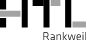
\includegraphics[height=1.5cm]{main/Logo1.png}
    \end{minipage}
    \hfill
    \raisebox{1.2cm}{ % << lift the center minipage
      \begin{minipage}[t]{0.3\textwidth}
        \raggedright
        \small
        \textbf{\Large HTBLuVA Rankweil} \\
        Höhere Lehranstalt für \\
        Elektronik und Technische Informatik
      \end{minipage}
    }
    \hfill
    \begin{minipage}[t]{0.3\textwidth}
      \flushright
      
\includegraphics[height=1.5cm]{main/Logo2.png}
    \end{minipage}
  \end{center}
  \vspace{1.5cm} % spacing below the logos before title
  \begin{center}
    \textbf{\LARGE DIPLOMARBEIT} \\ [0.5em]
    \Large Fotobox
  \end{center}
}

\date{} % Remove date

\parindent0pt

% Code style
\definecolor{codegreen}{rgb}{0,0.6,0}
\definecolor{codegray}{rgb}{0.5,0.5,0.5}
\definecolor{codeorange}{rgb}{1.0,0.5,0}

\lstdefinestyle{csharp}{
    language=[Sharp]C,
    backgroundcolor=\color{gray!10},
    commentstyle=\color{codegreen},
    keywordstyle=\color{blue},
    numberstyle=\tiny\color{codegray},
    stringstyle=\color{codeorange},
    basicstyle=\ttfamily\small,
    breakatwhitespace=false,
    breaklines=true,
    captionpos=b,
    keepspaces=true,
    showspaces=false,
    showstringspaces=false,
    showtabs=false,
    tabsize=2,
    frame=single,
    framerule=0.5pt,
    morekeywords={partial, var, value, get, set, async, await}
}
\lstset{style=csharp}


\graphicspath{{images/}}


% Custom footer for the rest of the document
\fancypagestyle{plain}{  % The "plain" style is used for all pages after title
  \fancyhf{}  % Clear header and footer
  \renewcommand{\footrulewidth}{0.4mm}  % Adds a line above the footer
  \fancyfoot[R]{\thepage}  % Page number in the center of the footer
  \fancyfoot[L]{\small DA \textbar\ 2024/25 \textbar\ Fotobox \textbar\ Robin Ganahl}  % Custom text on the left
  \renewcommand{\headrulewidth}{0pt}  % No header line
}

\begin{document}


\maketitle

\vspace{-3cm}

% TODO: ersetzen durch die fertig zusamengabeuta fotobox
\begin{figure}[H]
  \centering
  
\includegraphics[width=0.6\textwidth]{images/mechanics/fotobox_frontplatte_v2.png}
\end{figure}

\thispagestyle{empty}  % No footer on the first page needs to come after \maketitle

\begin{table}[h!]
    \centering
    \begin{tabular}{l l l}
        \textbf{Ausgeführt im Schuljahr 2024|2025 von:} & & \textbf{Betreuer/in:} \\ 
        \\
        Robin Ganahl & 6/7ABELI & Diem Lukas, DI, BEd. \\ 
    \end{tabular}
\end{table}

\vspace{0.5cm} % Adds space between table and date
Rankweil, am \today
\\
\rule{\linewidth}{0.4mm}  % Creates a line that spans the entire width of the page

\begin{table}[h!]
    \centering
    \begin{tabular}{l @{\hspace{6cm}} l}  % Add horizontal space between the columns
        \textbf{Abgabevermerk:} & \\ 
        \\
        AA original, am 8. April 2025 & Diem Lukas, DI, BEd. \\ 
        \\
        AA digital, am 8. April 2025 & Plattform \\ 
    \end{tabular}
\end{table}

\newpage
\tableofcontents
\newpage

\pagestyle{plain}  % Use custom footer starting from this point

\section{Zusammenfassung}

\subsection{Aufgabenstellung}

Viele Fotobox-Programme sind entweder kostenpflichtig und oft sehr teuer, oder 
als Open-Source-Software verfügbar, aber technisch veraltet und schwer anpassbar.
Diese Einschränkungen machen es schwierig, eine kostengünstige und moderne
Lösung zu finden, die den aktuellen Anforderungen entspricht.
Daher habe ich mich entschieden, im Rahmen meines Maturaprojekts ein eigenes
Fotobox-Programm in C\# zu entwickeln und eine passende Fotobox-Hardware zu bauen.
Mein Ziel ist es, eine benutzerfreundliche, flexible und zeitgemäße Alternative
zu bestehenden Lösungen zu schaffen.

\subsection{Umsetzung}

Für die Umsetzung des Projekts habe ich eine moderne Fotobox-Software in C\# entwickelt,
welche auf einem Windows-PC verwendet werden kann. Die Software unterstützt sowohl Webcams,
beispielsweise die im Laptop integrierte Kamera, als auch professionelle Canon-Spiegelreflexkameras.
Die Fotobox-Hardware besteht aus einer hochwertigen Kamera und einem Laptop mit Touchscreen,
der sowohl zur Bedienung als auch zur Verarbeitung der Bilder dient. 
Für die Benutzerinteraktion wurde eine intuitive Oberfläche mit großen,
leicht verständlichen Buttons entwickelt, um die Bedienung so einfach wie
möglich zu gestalten. Die erstellten Bilder können anschließend direkt
ausgedruckt oder über eine Cloud-Anbindung auf einen Server hochgeladen werden.
Von dort aus können sie bequem auf ein Smartphone heruntergeladen werden.

\subsection{Ergebnisse}

Das Projekt führte zu einer voll funktionsfähigen Fotobox, die eine
benutzerfreundliche und moderne Lösung für Veranstaltungen bietet.
Die Software ermöglicht die Steuerung einer Kamera, das Aufnehmen,
Speichern und Teilen von Fotos sowie den direkten Druck. Dank einer intuitiven
Oberfläche ist die Bedienung einfach und effizient.
Ein besonderer Fokus lag auf der Modularität: Das System kann problemlos
um neue Funktionen, wie Filter oder zusätzliche Hardware erweitert werden.
Zudem wurde eine Cloud-Anbindung integriert, sodass Nutzer ihre Fotos direkt
auf ihr Smartphone herunterladen können. Insgesamt entstand eine kostengünstige,
flexible und zeitgemäße Alternative zu bestehenden Fotobox-Lösungen.

\graphicspath{{images/program}}

\section{Software Architektur}

\begin{figure}[H]
    \centering
    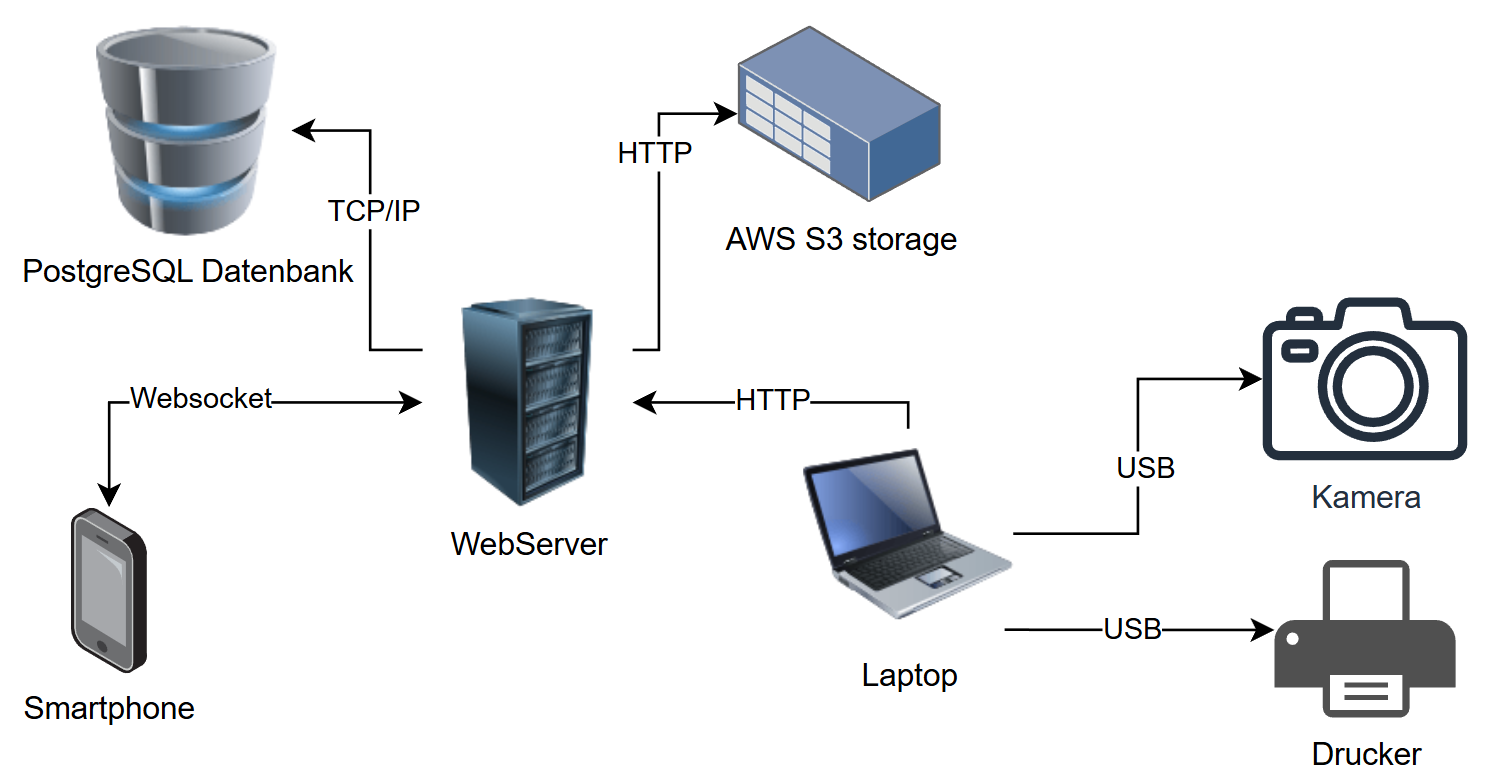
\includegraphics[width=0.7\textwidth]{system_architektur.png}
    \caption{Übersicht über die Fotobox-Software}
    \label{fig:system_architektur}
\end{figure}

% In diesem Kapitel wird das Programm beschrieben, welches die Fotobox steuert.
% Zuerst grober aufbau mitteld diagramm und beschreibung einzelner komponenten.
% Dann in späteren kapiteln genauere beschreibung.

Das gesamte Fotoboxsystem besteht aus mehreren Komponenten, die möglichst nahtlos
miteinander Arbeiten, um dem Benutzer eine einfache und intuitive Bedienung
zu ermöglichen. 

Im Zentrum steht das Windows-Programm, das die Steuerung der Kamera und des
Druckers übernimmt. Es zeigt das Livebild der Kamera auf dem Laptop an,
verarbeitet die aufgenommenen Bilder und sendet sie an den Webserver.

Ein weiterer Bestandteil ist der Webserver, welcher einerseits für die 
Endbenutzer die hochgeladenen Bilder zum Download bereitstellt, und andererseits
für den Administrator eine Weboberfläche zur Verwaltung seiner registrierten 
Fotoboxen bietet. Der Webserver kommuniziert außerdem auch mit der
Datenbank und dem AWS S3 Cloud Storage, um die Bilder zu speichern und
zu verwalten.

Das Zusammenspiel dieser Komponenten sowie deren genaue Funktionsweise werden
in den folgenden Kapiteln im Detail erläutert.

\newpage

\subsection{Desktop Applikation}

In dem folgenden Kapitel wird die Desktopapplikation 

\begin{figure}[H]
    \centering
    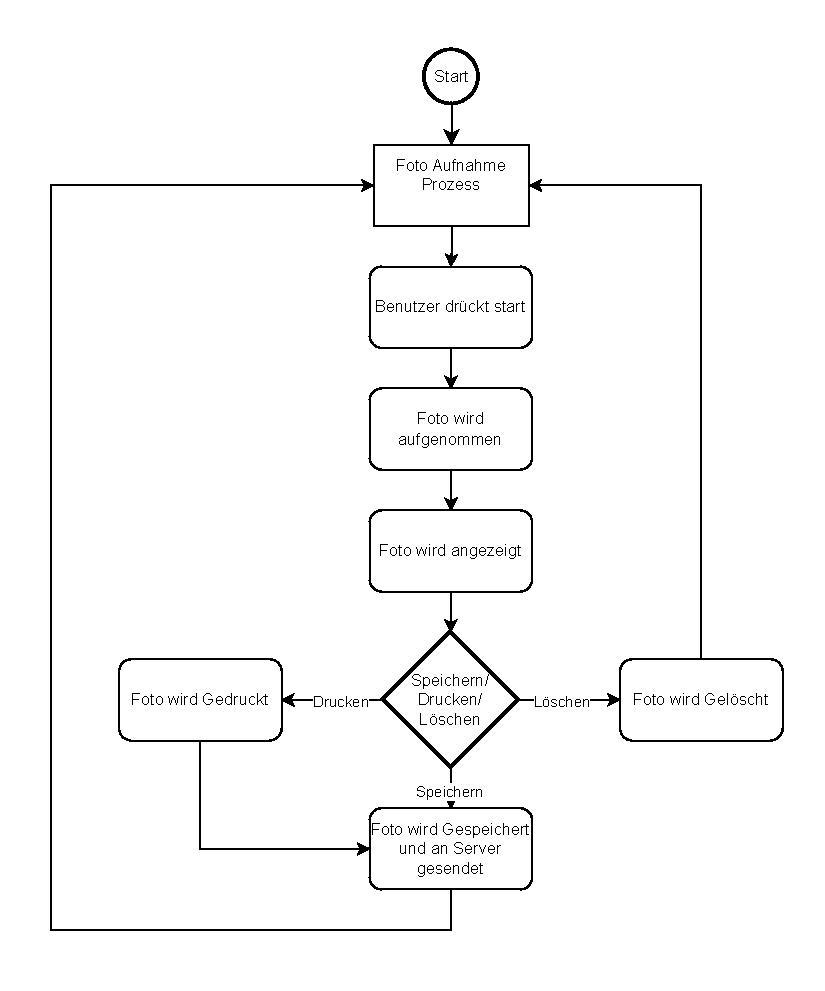
\includegraphics[width=0.75\textwidth]{Ablauf_Foto_Aufnehmen.drawio.pdf}
    \caption{Ablaufdiagramm der Fotoaufnahme.}
    \label{fig:Ablauf_Foto_Aufnehmen}
\end{figure}

In der \autoref{fig:Ablauf_Foto_Aufnehmen} ist der Ablauf der Fotoaufnahme dargestellt.
Wenn der Benutzer auf den Auslöser drückt, wird ein Foto aufgenommen.
Anschließend wird das Bild auf dem Laptop angezeigt, und der Benutzer hat die Möglichkeit,
auszuwählen, ob das Foto gespeichert, bzw. gedruckt werden soll, oder nicht.

\newpage

\subsection{Webserver}

\newpage

\subsection{Verwendete Technologien}

In dem folgenden Kapitel werden die Technologien beschrieben, welche ich verwendet habe,
um das Projekt zu realisieren.

\subsubsection{Programmiersprache}
C\# ist eine moderne, objektorientierte Programmiersprache, die von Microsoft entwickelt wurde.
Ich habe, da ich bereits Erfahrung mit C\# habe und diese Sprache sehr viel Flexibilität bietet,
einerseits für die Entwicklung von Desktopanwendungen, als auch für die Entwicklung
von Webservern und sogar Webanwendungen, entschieden.

\subsubsection{ASP.NET Core}
ASP.NET Core ist ein plattformunabhängiges, modulares und leistungsfähiges
Framework zur Entwicklung von Webanwendungen und APIs. Es wurde als Nachfolger
von ASP.NET entwickelt und bietet eine moderne Architektur sowie eine hohe
Performance. Im Projekt dient ASP.NET Core als Grundlage für die Serveranwendung,
welche für die Verwaltung der Benutzer und der aufgenommenen Bilder verantwortlich ist.
Durch die integrierte Unterstützung von Abhängigkeiten, Authentifizierung und RESTful
APIs war ASP.NET Core eine ideale Wahl für die Backend-Entwicklung.

\subsubsection{Blazor}
Blazor ist ein Framework zur Erstellung interaktiver Webanwendungen mit C\#,
das im Rahmen von ASP.NET Core entwickelt wurde. Es ermöglicht die Entwicklung
von Web-UIs mit C\# statt JavaScript. In meinem Projekt habe ich Blazor WebAssembly
verwendet, um eine clientseitige Webanwendung zur Konfiguration und Gestaltung
der aufgenommenen Bilder umzusetzen. Diese Webanwendung läuft direkt im Browser
und kommuniziert über HTTP mit dem Backend.

\subsubsection{Entity Framework Core}
Entity Framework Core ist ein objekt-relationaler Mapper (ORM) für .NET.
Es erlaubt, Datenbankabfragen in C\# zu formulieren, wodurch die Interaktion
mit der Datenbank deutlich vereinfacht wird. In meinem Projekt verwende ich
Entity Framework Core zur Verwaltung und Persistierung von Benutzerdaten sowie
Bildinformationen. Die Verwendung eines ORM trägt außerdem zur Wartbarkeit und
Erweiterbarkeit der Anwendung bei.

\subsubsection{Canon EDSDK}
Zur Ansteuerung der Canon-Spiegelreflexkamera verwende ich das Canon EOS Digital
SDK (EDSDK). Dieses Software Development Kit ermöglicht es, über eine
USB-Verbindung Fotos aufzunehmen und Kameraeinstellungen zu verändern.
Die Integration dieser Schnittstelle in die Anwendung erlaubt es, Bilder direkt
aus der Anwendung heraus aufzunehmen und zu speichern.

\subsubsection{Windows Credential Manager}
Der Windows Credential Manager wird genutzt, um Anmeldedaten wie den Refresh-Token
nach Beenden der Anwendung sicher auf dem System zu speichern.
Dadurch können Benutzer auch nach einem Neustart der Anwendung
automatisch eingeloggt bleiben, ohne ihre Zugangsdaten erneut eingeben zu müssen.

%TODO: neuer name für kapitel
\subsection{Architektonische Konzepte}

In diesem Kapitel werden zentrale Entwurfskonzepte und Prinzipien vorgestellt,
die bei der Umsetzung der Anwendung eine wichtige Rolle gespielt haben.

\subsubsection{Dependency Injection und IoC}
Inversion of Control (IoC) ist ein Prinzip, bei dem die Steuerung über
die Erstellung und Verwaltung von Abhängigkeiten nicht vom Entwickler,
sondern vom Framework übernommen wird. In .NET wird dieses Prinzip durch
Dependency Injection (DI) umgesetzt. Alle Dienste und Komponenten werden im
sogenannten IoC-Container registriert und bei Bedarf automatisch bereitgestellt.
Diese Struktur verbessert die Testbarkeit und Modularität des Codes.

In dem folgenden Code Snippet wird gezeigt, wie eine Abhängigkei, hier die 
Drucker-Klasse in den IoC-Container registriert wird:

\begin{lstlisting}
builder.Services.AddSingleton<IPrinter, Printer>();
\end{lstlisting}    

Wenn die Printer-Klasse nun benötigt wird, kann sie einfach im Konstruktor
einer anderen Klasse injiziert werden:

\begin{lstlisting}
public class ImageManager(IPrinter printer)
{
    private readonly IPrinter _printer = printer;

    public async Task PrintAndSaveAsync(Image<Rgb24> image)
    {
            await SaveAsync(image);

            await printer.PrintAsync(image);
    }
}
\end{lstlisting}

Wenn nun diese \emph{ImageManager}-Klasse vom IOC Container instanziiert wird,
wird automatisch die Printer-Klasse mit übergeben. Bei diesem Beispiel, 
ist es noch sehr übersichtlich, da nur eine Abhängigkeit vorhanden ist.
Wenn jedoch mehrere Abhängigkeiten vorhanden sind, wird es schnell
unübersichtlich, was durch die Verwendung von Dependency Injection
deutlich vereinfacht wird. Außerdem wird das unnötige Erstellen und
Zerstören von Objekten vermieden, was die Performance der Anwendung
verbessert, da hier die Printer-Klasse nur einmal erstellt wird und
nicht bei jedem Aufruf der PrintAndSaveAsync-Methode neu instanziiert werden muss.

\subsubsection{ILogger und Serilog}

Für das Logging wurde das \texttt{ILogger\textless{}T\textgreater{}}-Interface
aus dem .NET Core Framework verwendet. Dieses Interface ermöglicht eine
einheitliche und flexible Protokollierung, bei der Logeinträge in
unterschiedlichen Formaten und über verschiedene Ausgabemedien
(z.\,B. Konsole, Datei oder Remote-Logging-Dienste) erzeugt werden können 
ganz ohne Anpassungen am Anwendungscode.

Die Bereitstellung des Loggers erfolgt über Dependency Injection.
Jede Klasse kann dadurch eine auf ihren Typ spezialisierte Instanz von
\texttt{ILogger\textless{}T\textgreater{}} erhalten. Das verbessert die
Nachvollziehbarkeit im Log, da jeder Eintrag eindeutig der Herkunftsklasse
zugeordnet werden kann.

Im folgenden Beispiel wird gezeigt, wie Logging in der \texttt{Printer}-Klasse
verwendet wird:

\begin{lstlisting}
public class Printer(ILogger<Printer> logger)
{
    private readonly ILogger<Printer> _logger = logger;

    public Task PrintAsync(Image<Rgb24> image)
    {
        // Drucken des Bildes

        _logger.LogInformation(
            "Bild erfolgreich gedruckt: {imageName}", image.Name);
    }
}
\end{lstlisting}

Zur Ausgabe der Logeinträge wird Serilog als Logging-Provider verwendet.
Die Konfiguration erfolgt bei der Erstellung des Host-Builders:

\begin{lstlisting}
var logger = new LoggerConfiguration()
    .Enrich.FromLogContext()
    .Enrich.WithEnvironmentName()
    .Enrich.WithMachineName()
    .Enrich.WithProperty("Source", "UI")
    .WriteTo.Seq("http://localhost:5341")
    .CreateLogger();

builder.Logging.AddSerilog(logger);
\end{lstlisting}

Die Logs können so flexibel an verschiedene Ziele weitergeleitet werden etwa,
in die Konsole, in lokale Dateien oder an zentrale Logging-Dienste wie Seq.
Dies ermöglicht eine kontinuierliche Überwachung des Systemverhaltens zur
Laufzeit und eine gezielte Analyse im Fehlerfall.

Insgesamt trägt dieses Logging-Konzept entscheidend zur Wartbarkeit und Fehlersuche bei,
da relevante Abläufe und Probleme nachvollziehbar und strukturiert dokumentiert werden.

\section{Installation und Konfiguration}

Da das Projekt aus mehreren Komponenten besteht, einerseits die Desktopanwendung,
welche auf dem Windows Laptop installiert wird, und dem Webserver, welcher
auf einem aus dem öffentlichen Internet zugänglichen Server installiert wird,
für den Endnutzer ist jedoch nur die Installation auf dem Windows Laptop notwendig.
Die Installation auf dem Server sollte normalerweise nicht notwendig sein, wen
mein Dienst verwendet wird.

\subsection{Installation des Webservers}


\graphicspath{{images/mechanics}}

\section{Mechanik}

In der Nächsten Sektion wird die Mechanik der Fotobox beschrieben.
Die Mechanik ist ein sehr wichtiger Teil der Fotobox, da sie das erste
ist, was der Endbenutzer sieht. Sie sollte daher ansprechend und so stabil
aufgebaut sein, dass sie auch bei häufigem Transport nicht beschädigt wird.
Daher werde ich nun erläutern, warum ich mich für das aktuelle Design entschieden habe
und welche Probleme ich dabei hatte.

\subsection{Design}

Da das Design der Fotobox sehr wichtig ist, habe ich verschiedene Designs ausprobiert.
Der Weg, welcher zum schlussendlichen Design geführt hat, wird in Folgendem Unterkapitel beschrieben.

\begin{figure}[H]
    \centering
    
\includegraphics[width=1\textwidth]{fotobox_frontplatte_v1.png}
    \caption{Die erste Version der Frontplatte.}
    \label{fig:frontplatte_v1}
\end{figure}

In der \autoref{fig:frontplatte_v1} ist die erste Version der Frontplatte zu sehen.
Bei diesem Design, habe ich mich an schon am Markt erhältlichen Fotoboxen orientiert.
In den löchern eins und zwei sollten jeweils ein Blitz und eine LED Lampe platziert werden,
in dem mittleren Loch mit der Nummer drei sollte die Kamera platziert werden.

Jedoch hat sich herausgestellt, dass diese Design, durch die seitliche Platzierung des Blitzes
das Bild nicht einheitlich ausleuchtet, und einen seitlichen Schatten hinter dem 
Motiv wirft. Was die Qualität der Bilder, wie in \autoref{fig:seitlicher_blitzt}
zu sehen ist, deutlich verringert, da das Bild auch nicht einheitlich ausgeleuchtet wird.

\newpage
\begin{figure}[H]
    \centering
    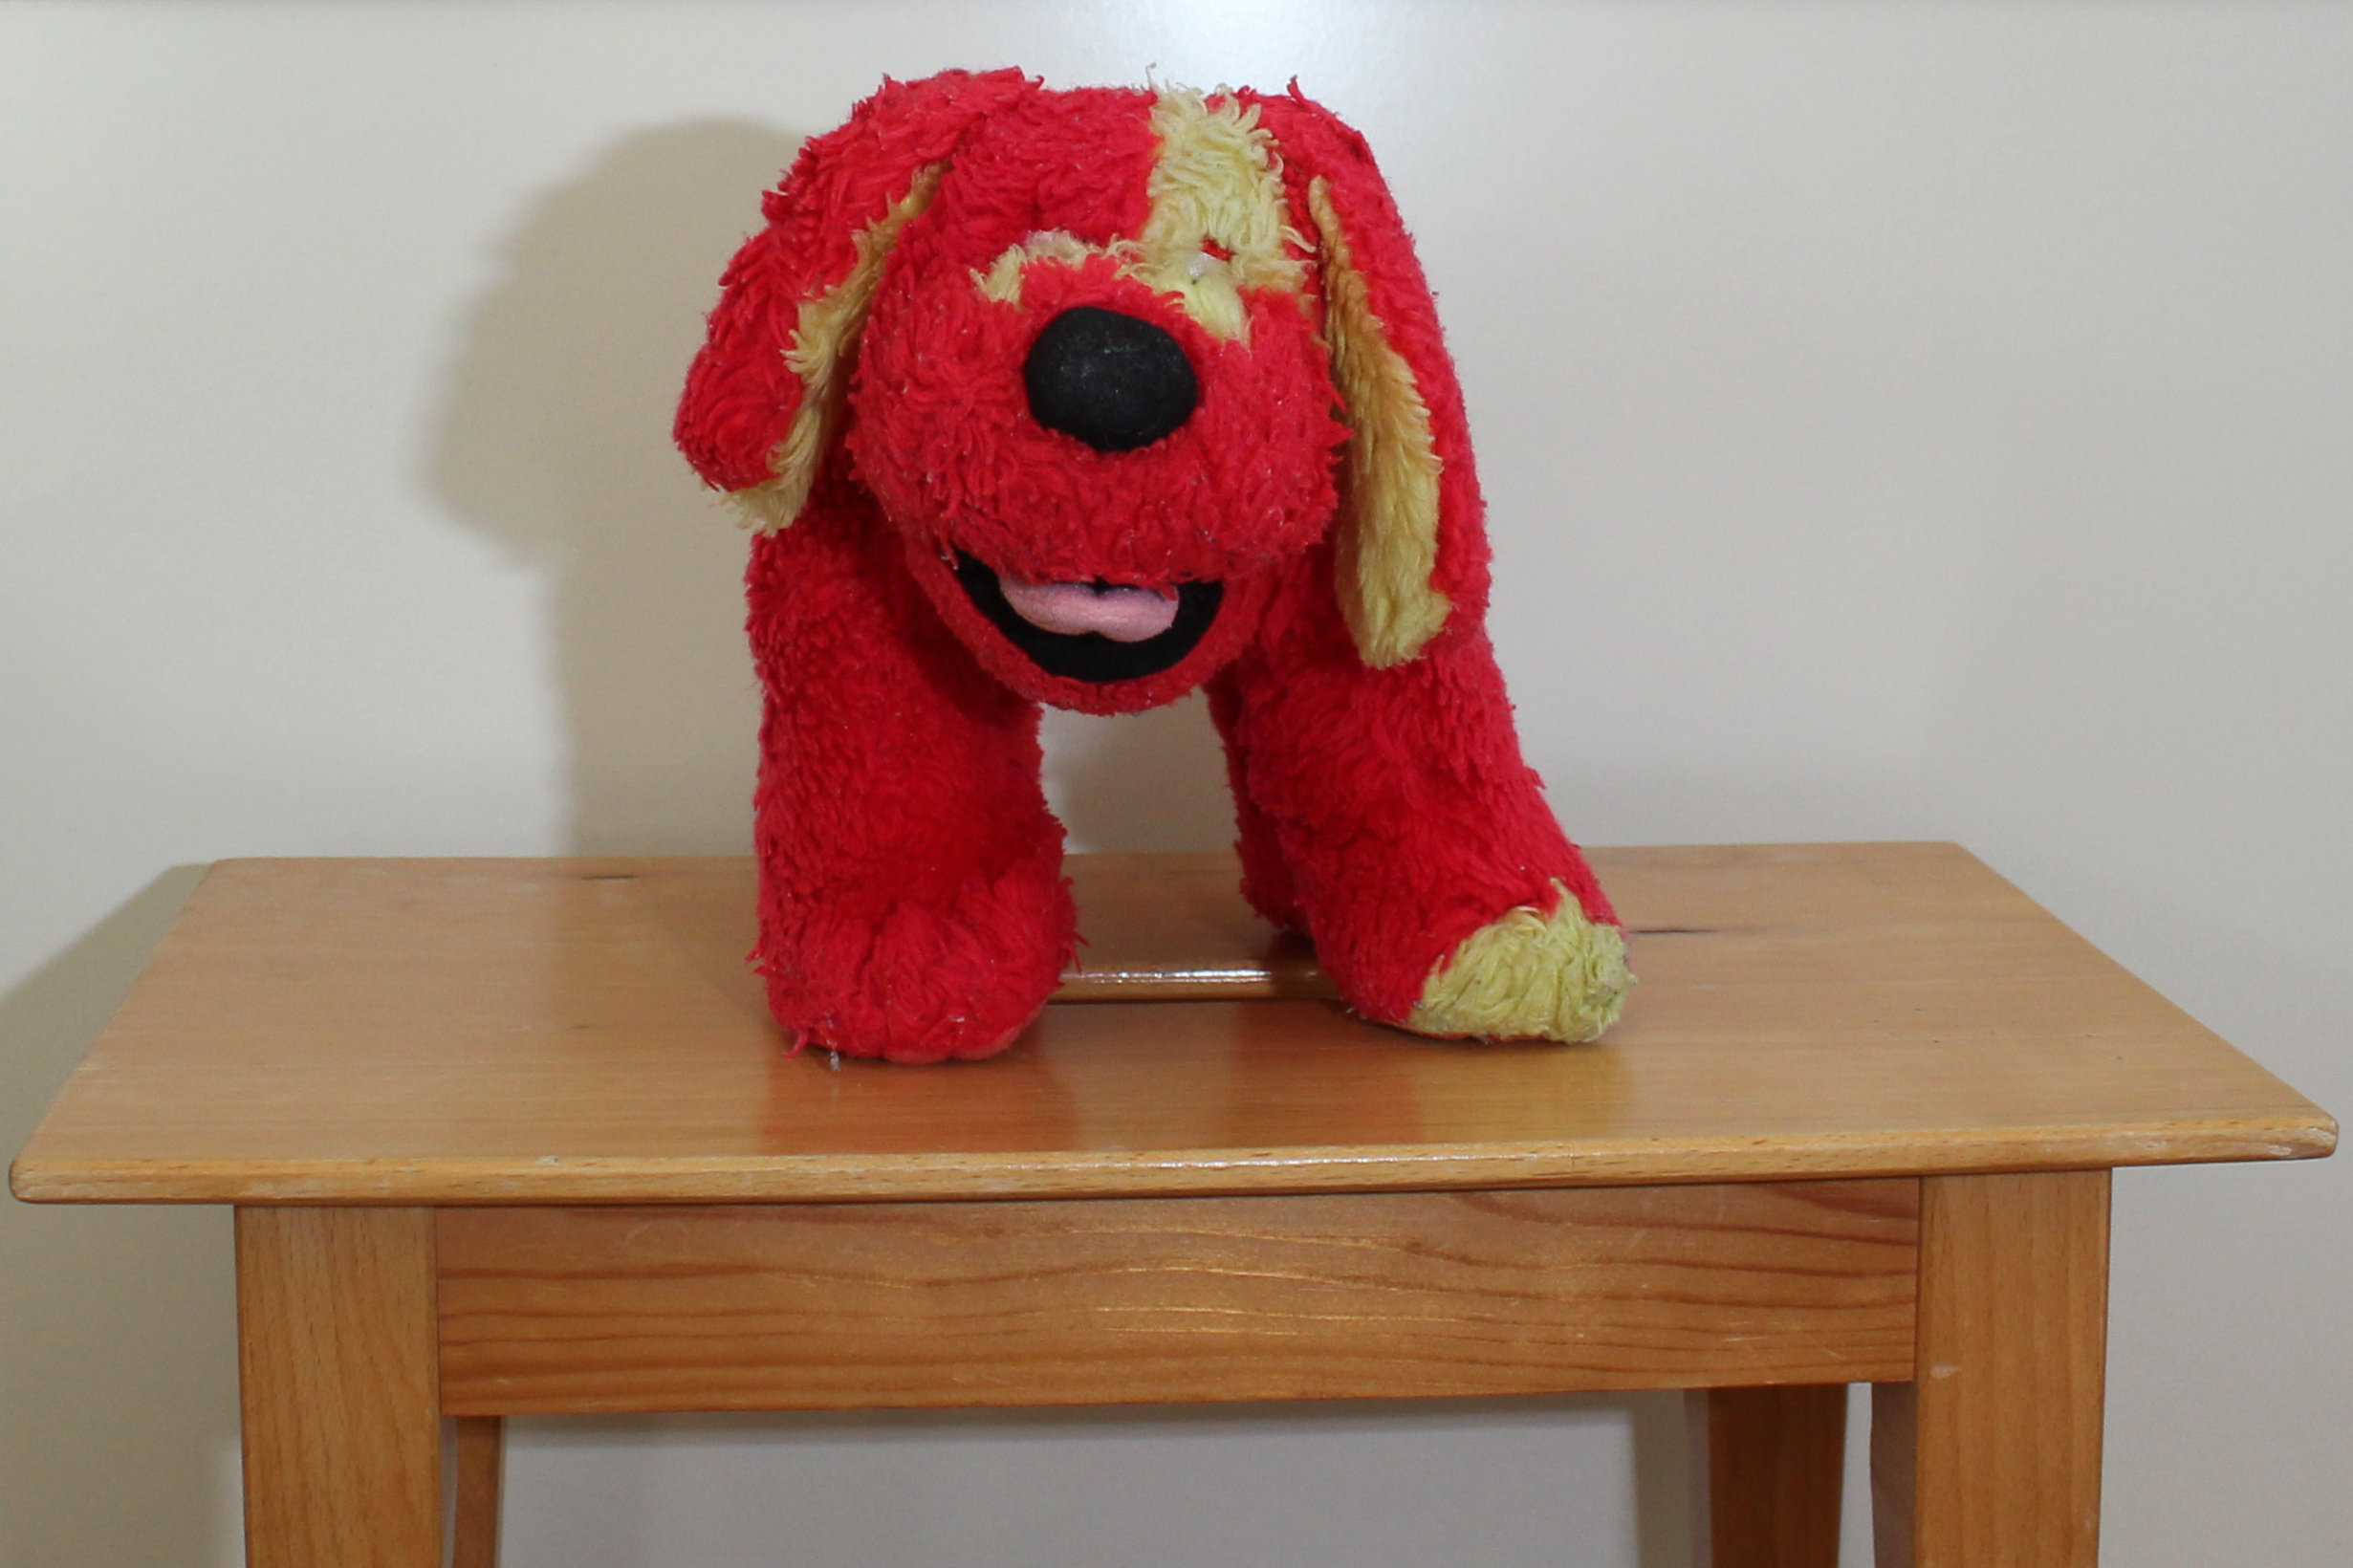
\includegraphics[width=0.8\textwidth]{blitz_seitlich.JPG}
    \caption{Beispielbild mit seitlichem Blitz.}
    \label{fig:seitlicher_blitzt}
\end{figure}

In der \autoref{fig:seitlicher_blitzt} ist zu sehen, dass durch die seitliche Platzierung des Blitzes 
auf der linken Seite neben dem Motiv ein Schatten entsteht. Dieser Schatten ist unerwünscht und sollte
durch ein zentrales Blitzlicht vermieden werden.

\begin{figure}[H]
    \centering
    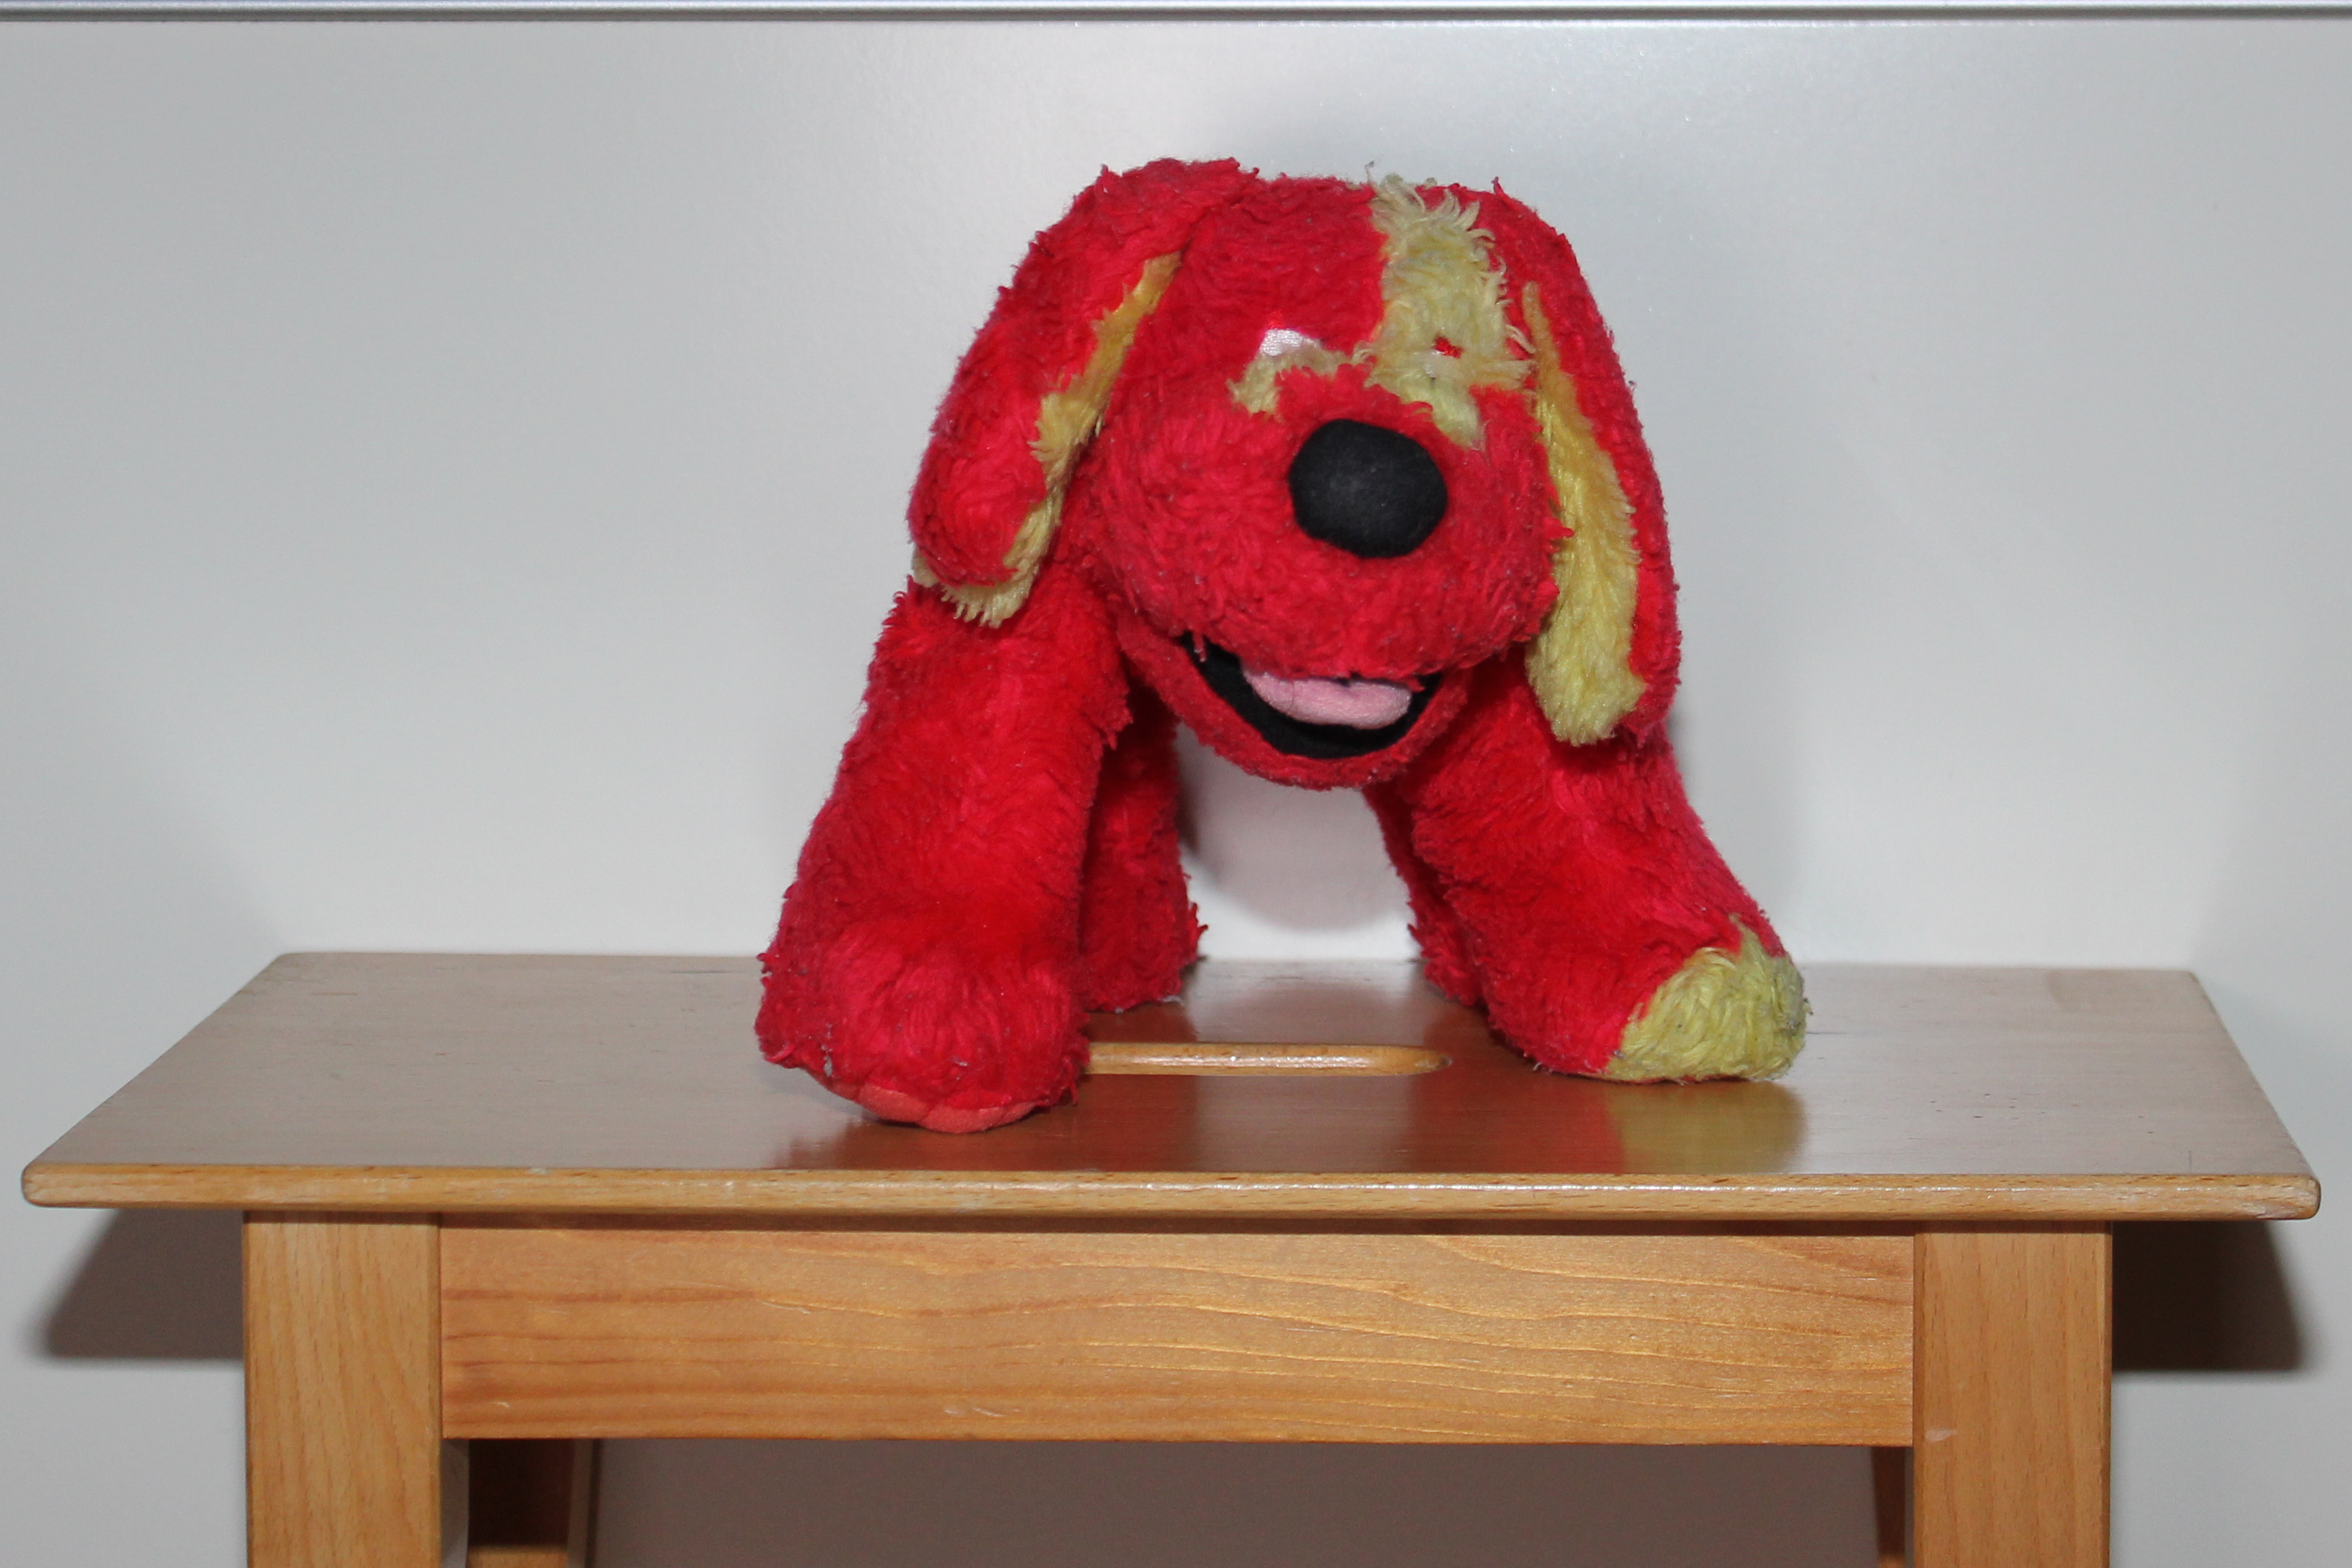
\includegraphics[width=0.8\textwidth]{blitz_vorne.JPG}
    \caption{Beispielbild mit zentralem Blitz.}
    \label{fig:zentraler_blitz}
\end{figure}

In der \autoref{fig:zentraler_blitz} ist zu sehen, dass durch die zentrale Platzierung des Blitzes,
das Bild deutlich besser ausgeleuchtet ist und keine seitlichen Schatten entstehen.
Darum habe ich mich dazu entschieden, das Design noch einmal zu überarbeiten und
den Blitzt zentral über der Kamera zu platzieren.

\newpage

Hier in \autoref{fig:frontplatte_v2} ist das überarbeitete Design zu sehen.
Im Gegensatz zur ersten Version, ist das neue Design 
nun höher, wie breit, wodurch es möglich ist, den Blitzt oberhalb der Kamera in 
Öffnung eins zu platzieren. In den Öffnungen zwei und drei sind die LED Lampen,
durch die auch bei der Vorschau, obwohl die Lichtquellen neben der Kamera sind,
eine symmetrische Beleuchtung des Motivs gewährleistet ist.

\begin{figure}[H]
    \centering
    
\includegraphics[width=0.75\textwidth]{fotobox_frontplatte_v2.png}
    \caption{Die erste Version der Frontplatte.}
    \label{fig:frontplatte_v2}
\end{figure}

Dieses Design bringt zudem weitere Vorteile mit sich. Besonders hervorzuheben
ist die Tatsache, dass die Form der Fotobox einem menschlichen Gesicht ähnelt.
Dies hat einen positiven psychologischen Effekt auf die Nutzerinnen und Nutzer:
Menschen fühlen sich in der Regel wohler und entspannter, wenn sie das Gefühl
haben, jemandem ins Gesicht zu blicken, anstatt lediglich vor einer anonymen,
leblosen Holzbox zu stehen. Die vertraute, „menschliche“ Gestaltung kann
Hemmschwellen abbauen und dazu beitragen, dass sich die Personen natürlicher und
ungezwungener vor der Kamera verhalten. Dadurch entstehen oft authentischere und
ausdrucksstärkere Fotos, was den Gesamteindruck und die Nutzererfahrung der Fotobox
deutlich verbessert.

\newpage

\subsection{Zusammenbau}

Im folgenden Kapitel wird der Zusammenbau der Fotobox beschrieben.
Da die Fotobox aus mehreren Teilen besteht, welche alle zuerst Zugeschnitten,
und alle nötigen Öffnungen gebohrt und gefräst werden müssen.

\subsubsection{Rohmaterial}

Das Rohmaterial, für welches ich mich entschieden habe, ist 18 mm dickes buchen
Leimholz, wie in \autoref{fig:rohmaterial} zu sehen ist.

\begin{figure}[H]
    \centering
    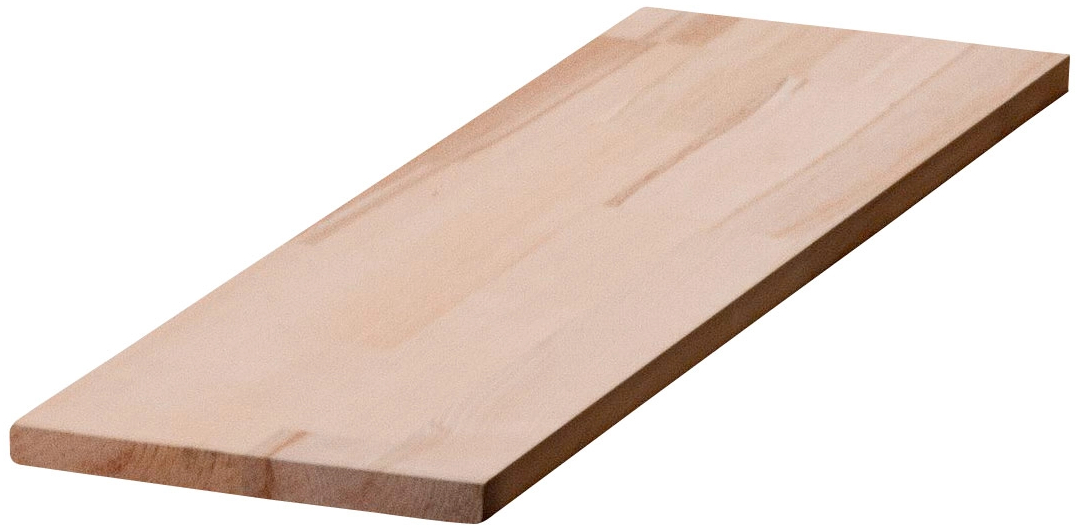
\includegraphics[width=0.75\textwidth]{rohmaterial.JPG}
    \caption{Das Rohmaterial der Fotobox.}
    \label{fig:rohmaterial}
\end{figure}

Ich habe mich für Leimholz aus Buche entschieden, da es durch die Verleimung der
einzelnen Holzlamellen eine hohe Formstabilität aufweist und sich kaum verzieht.
Zudem ist Buche ein sehr hartes Holz, wodurch die Box sehr stabil ist.
Jedoch ist Buche durch diese Eigenschaften auch schwerer zu verarbeiten,
als ein weicheres Holt und durch das höhere Gewicht, wird die Box auch schwerer.

\newpage

\subsubsection{Zuschnitt}

Zuerst sollten aus den beiden Platten mit den Maßen 2000 mm x 300 mm x 18 mm und 
2000 mm x 500 mm x 18 mm die einzelnen Teile der Fotobox auf der Kreissäge
zugeschnitten werden. In der Abbildung \autoref{fig:zuschnitt_mit_kreissaege} ist der grobe 
Zuschnitt der Platten auf der Kreissäge zu sehen.

\begin{figure}[H]
    \centering
    \includegraphics[width=0.75\textwidth]{zuschnitt_mit_kreissaege.JPG}
    \caption{Der Zuschnitt der Platten auf der Kreissäge.}
    \label{fig:zuschnitt_mit_kreissaege}
\end{figure}

Nach dem ersten groben Zuschnitt, wurde das Kreissägeblatt auf 45° gestellt, um
die kanten der Platten mit einer Fase zu versehen. Durch diese Fase, können die Platten
wie in \autoref{fig:fotobox_kanten} zu sehen ist, besser zusammengefügt werden.

\begin{figure}[H]
    \centering
    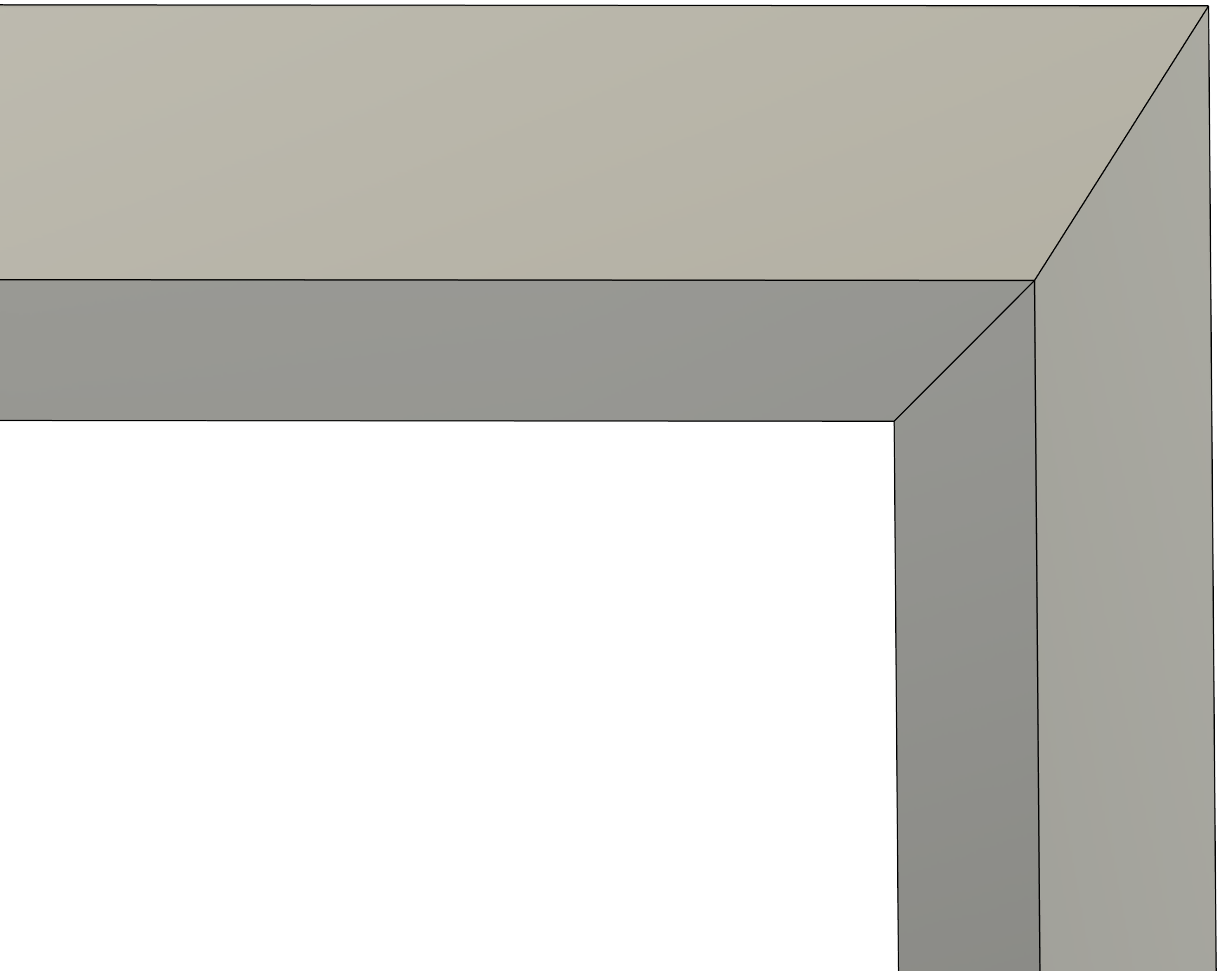
\includegraphics[width=0.5\textwidth]{fotobox_kanten.png}
    \caption{Zusammenfügen der Platten.}
    \label{fig:fotobox_kanten}
\end{figure}

Was erstens die Stabilität der Box erhöht und zweitens die Optik verbessert. 
Außerdem, wurde bei diesem Zweiten zuschnitt, auch darauf geachtet, dass die
Platten genau aneinander passen, da beim ersten Zuschnitt nur grobe Maße
genommen wurden.

\newpage

Nach dem alle Platten auf die richtige Größe zugeschnitten wurden und durch
Zusammensetzen, wie in \autoref{fig:fotobox_zusamensetzen_test}, der Box überprüft
wurde, dass die Platten auch ohne Lücken aneinander passen, wurden die Öffnungen
für die Kamera, den Blitz und die LED Lampen gefräst und gebohrt.

\begin{figure}[H]
    \centering
    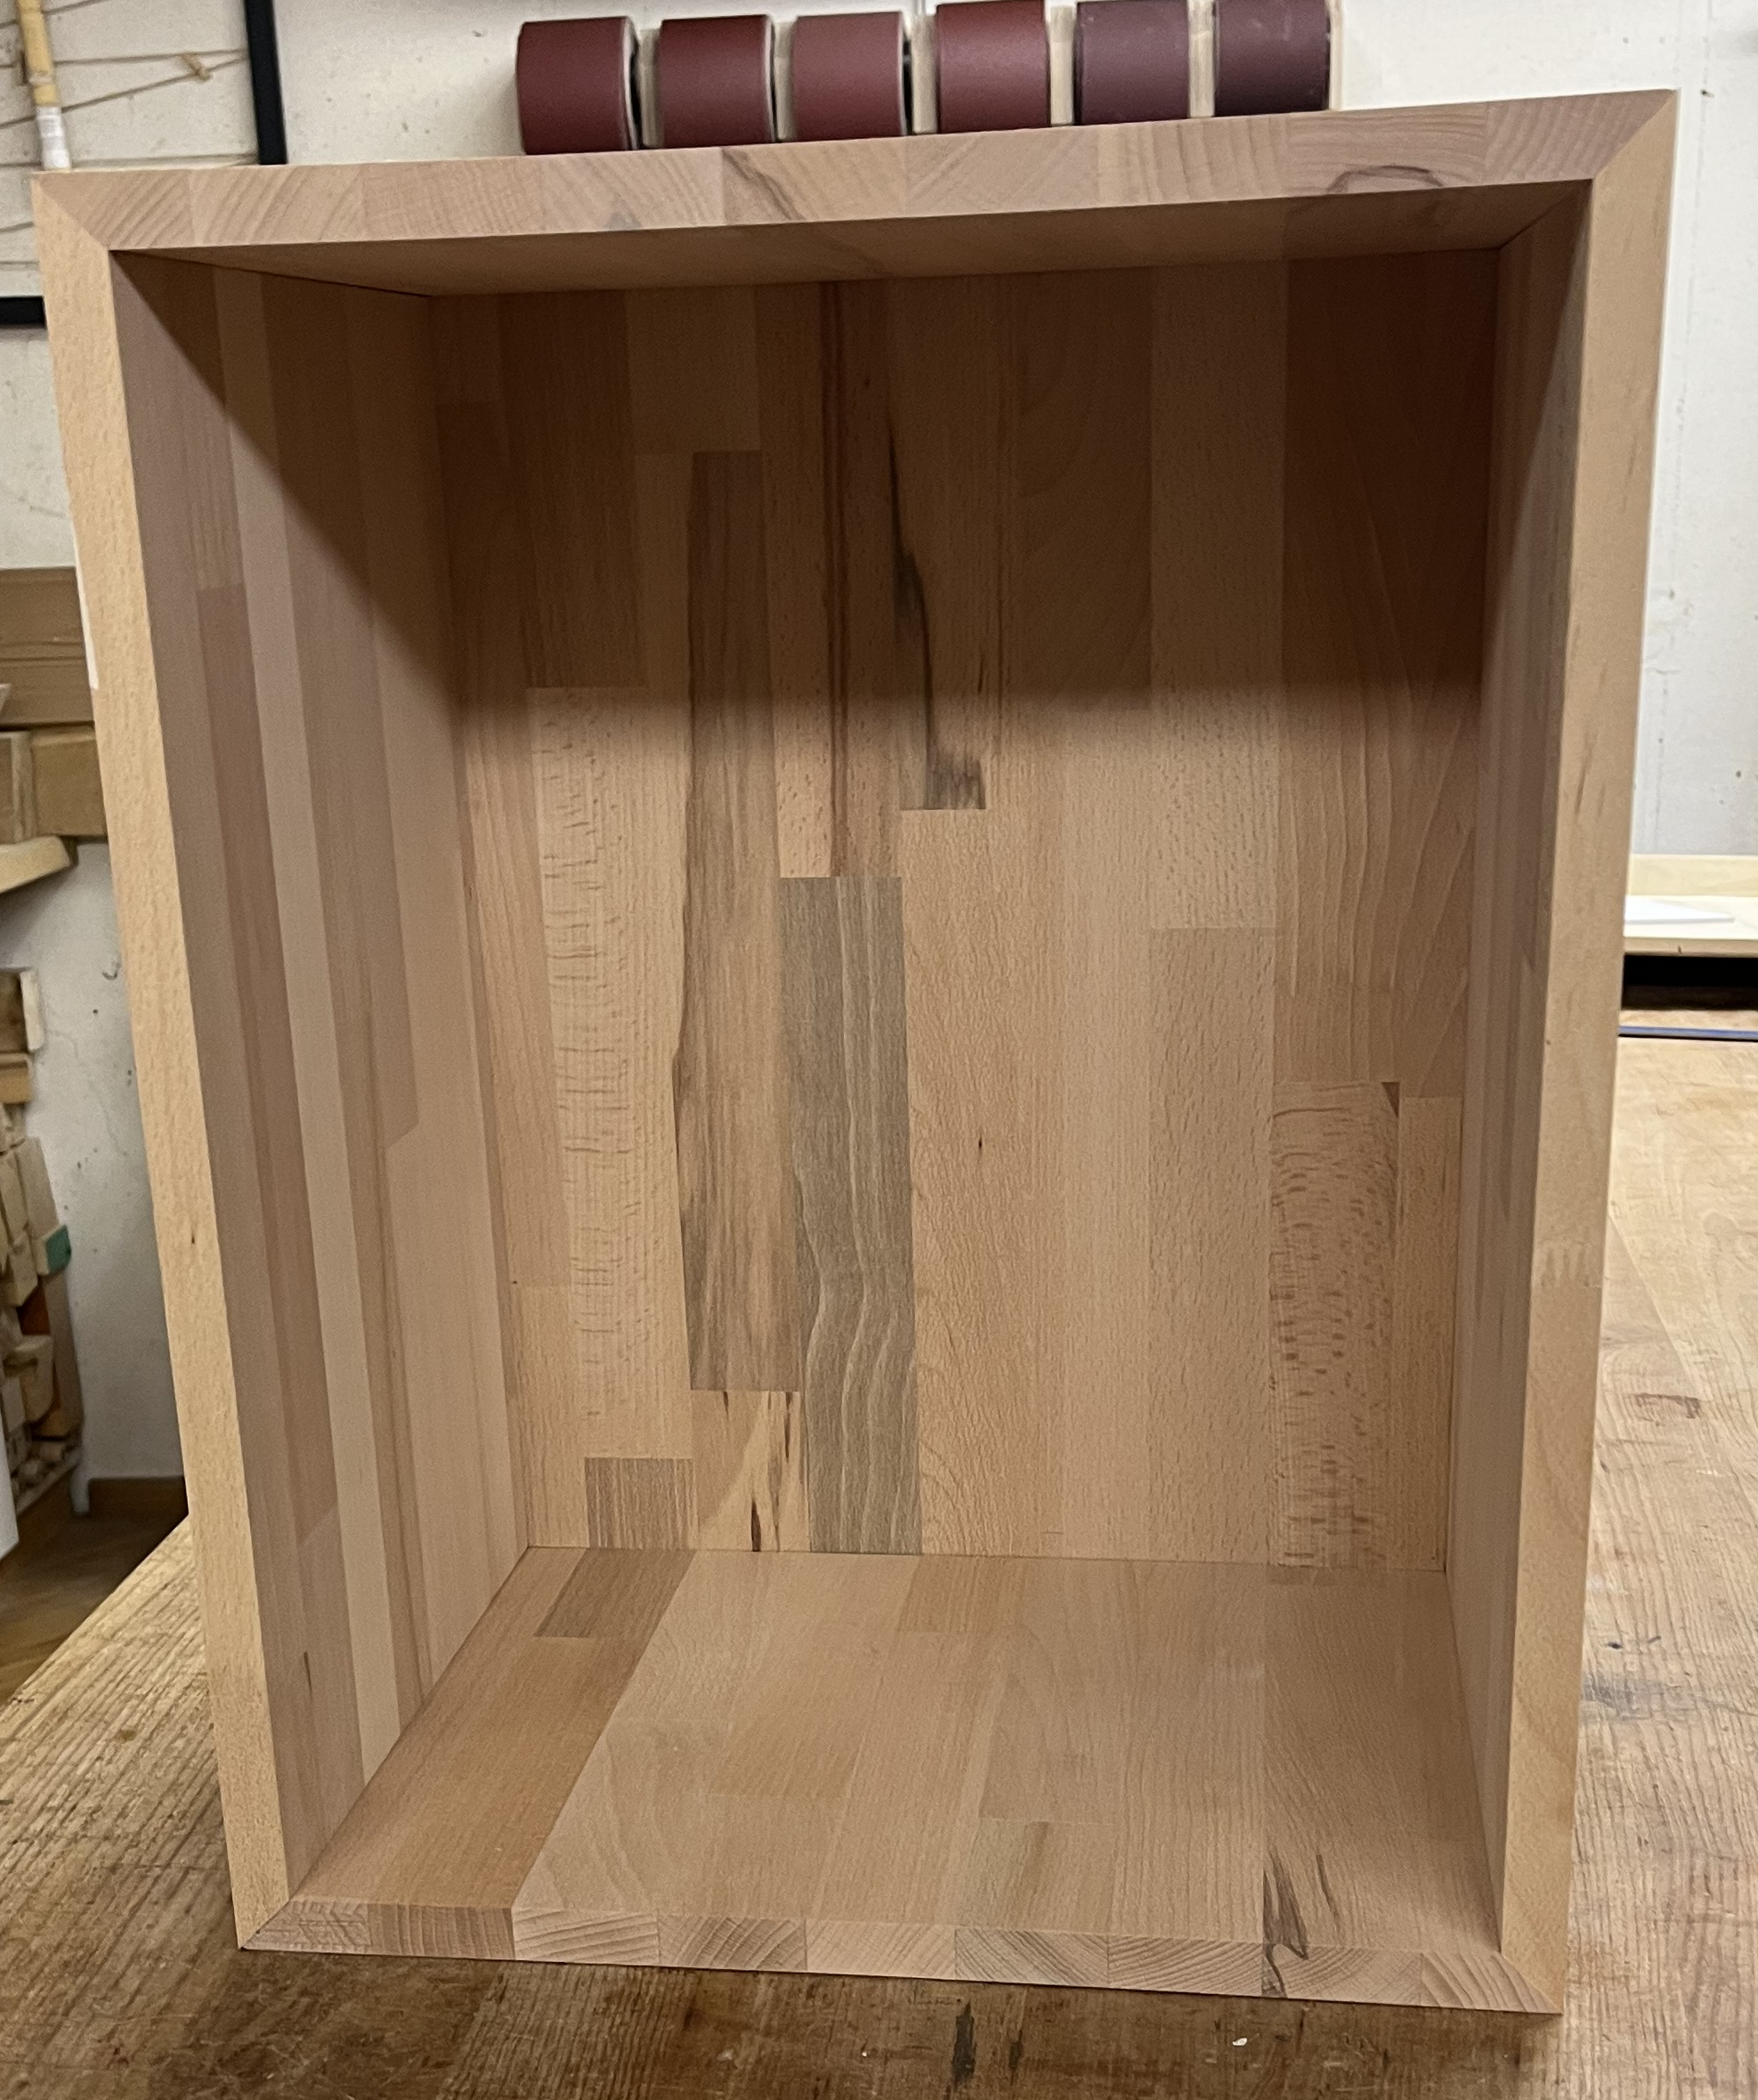
\includegraphics[width=0.6\textwidth]{fotobox_zusamensetzen_test.JPG}
    \caption{Überprüfen der Platten auf Passgenauigkeit der Platten.}
    \label{fig:fotobox_zusamensetzen_test}
\end{figure}

Um die Runden Öffnungen für die Kamera, die LED Lampen zu bohren, wurde die Frontplatte
auf der Standbohrmaschine eingespannt, und wie in \autoref{fig:fotobox_loch_saegen} zu sehen ist,
wurde mit einer Lochsäge die Öffnung für die Kamera und die LED Lampen gebohrt.

\begin{figure}[H]
    \centering
    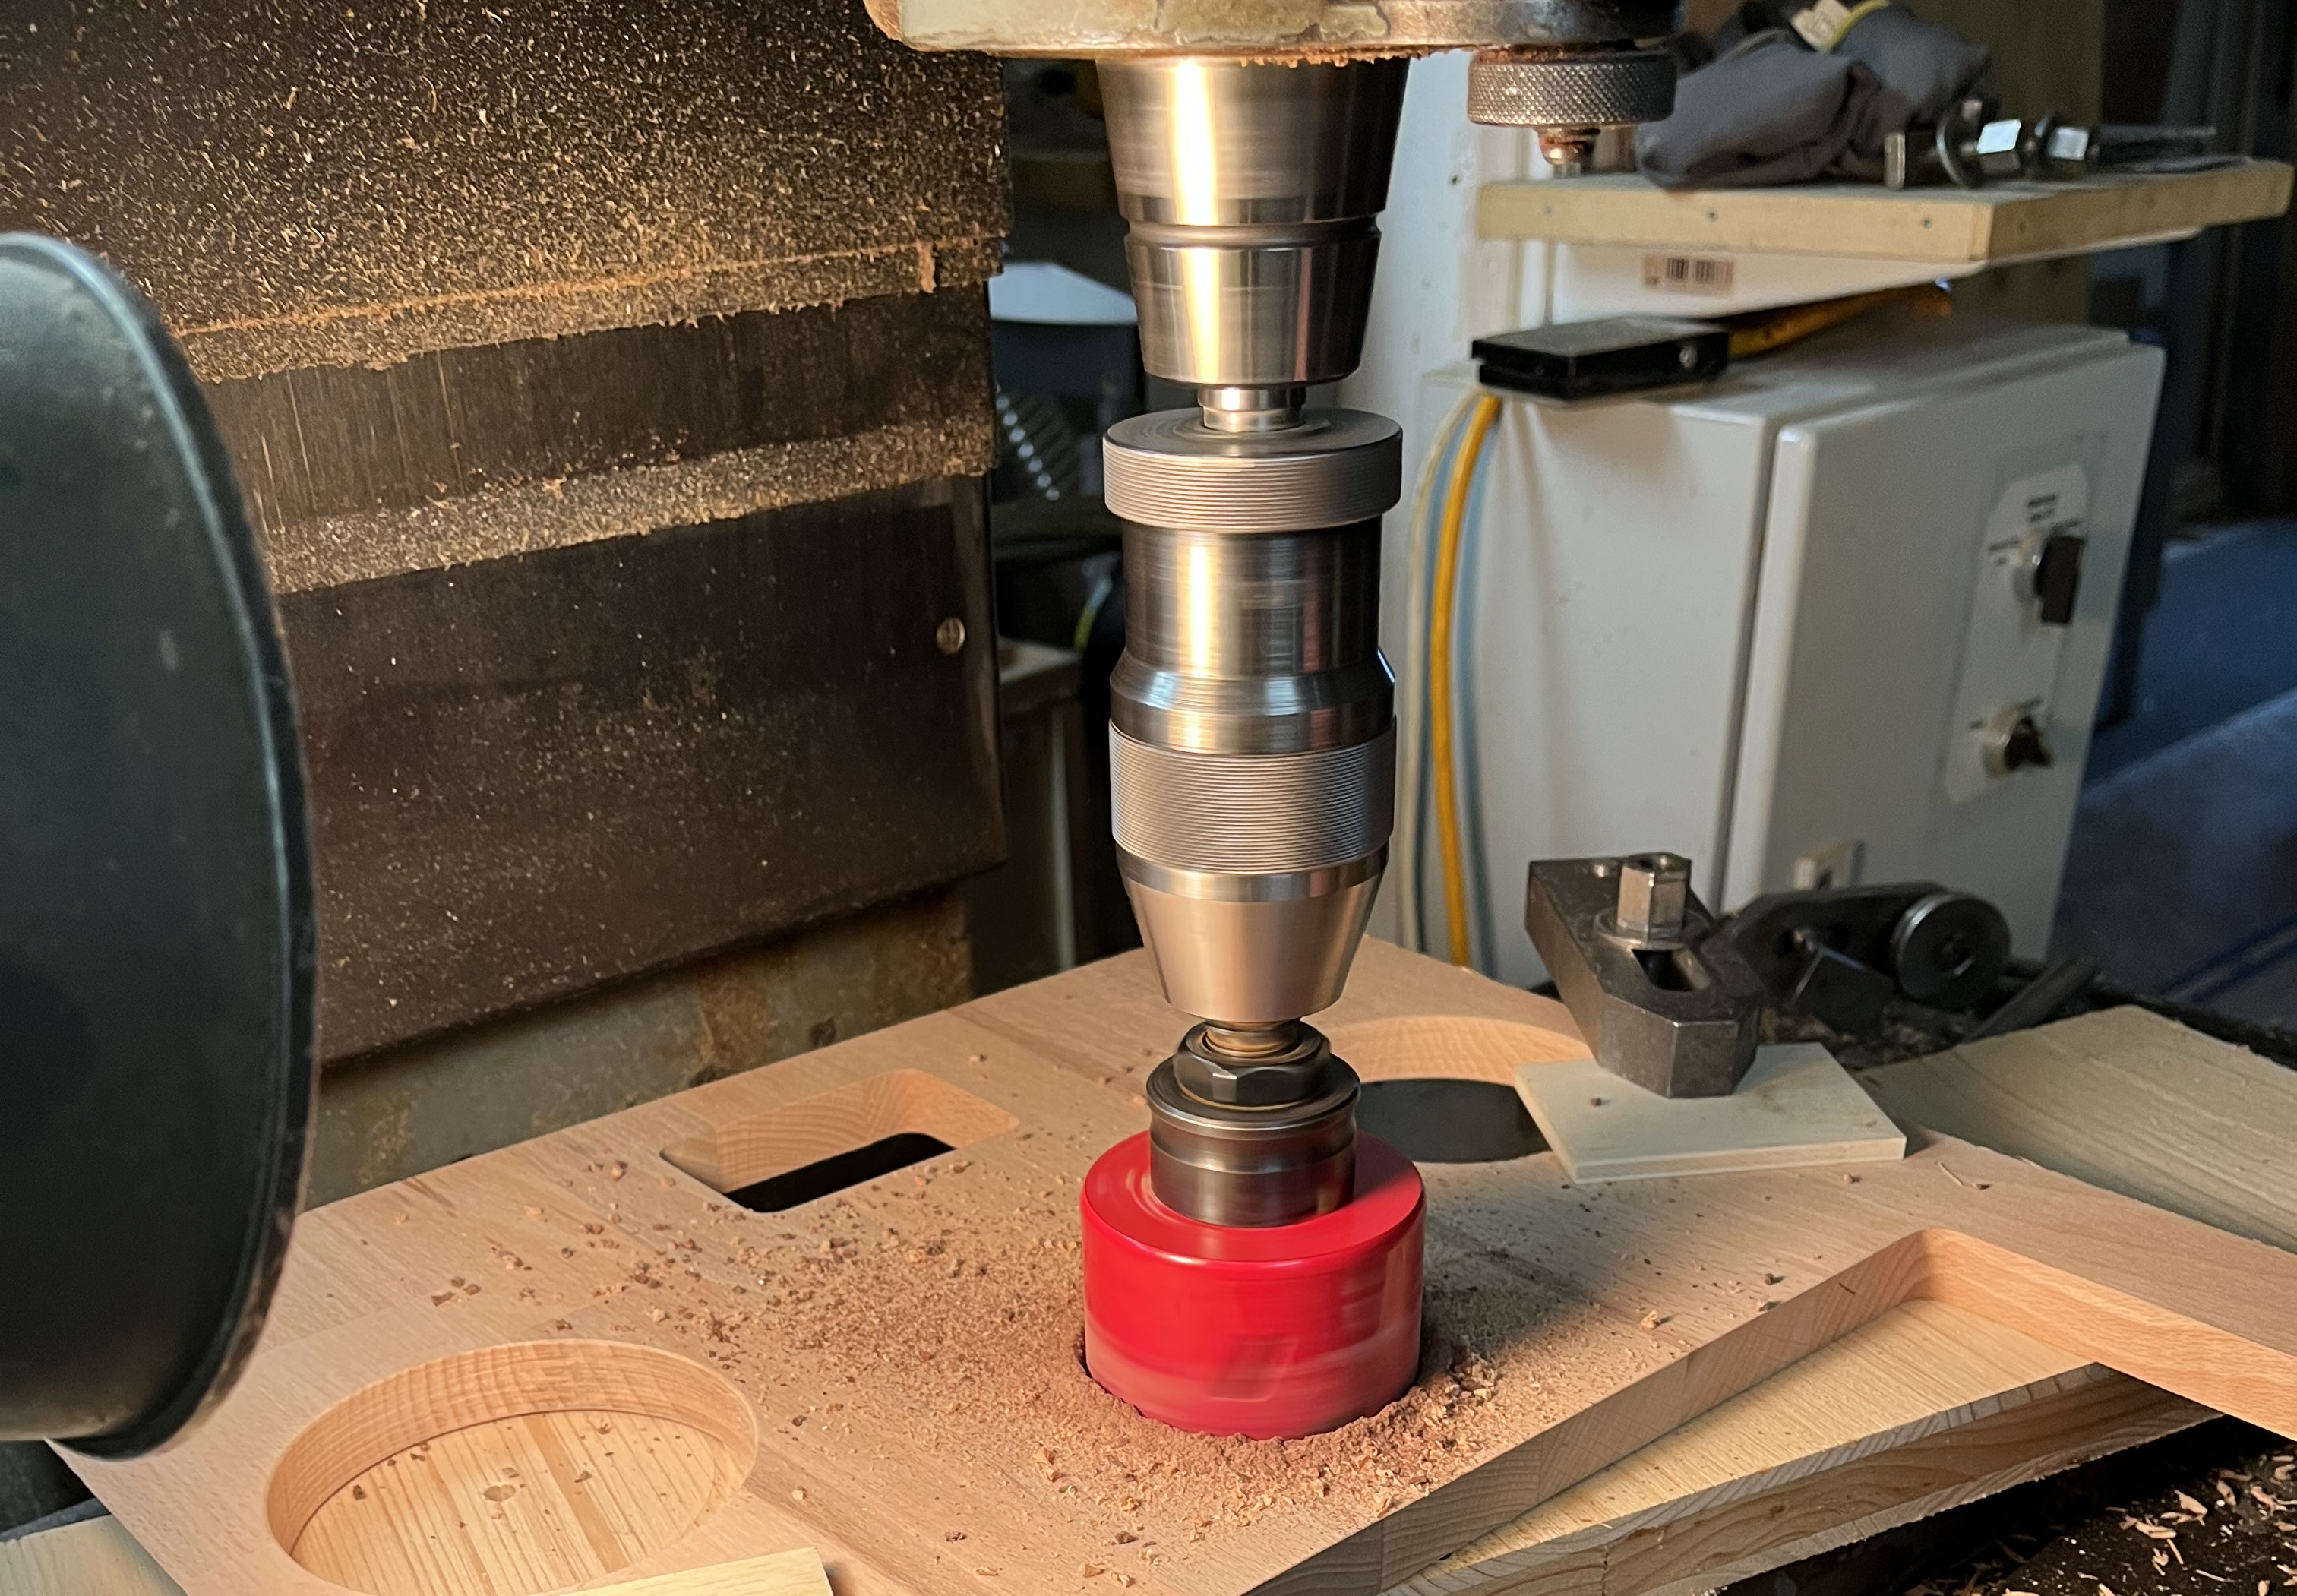
\includegraphics[width=0.75\textwidth]{fotobox_loch_saegen.JPG}
    \caption{Die Standbohrmaschine mit der Lochsäge.}
    \label{fig:fotobox_loch_saegen}
\end{figure}

Um die Öffnungen für den Blitz und Laptop auszuschneiden, wurde die Fräse verwendet.
Dazu wurde die Frontplatte auf der Fräse eingespannt und wie in
\autoref{fig:fotobox_fraesen} zu sehen ist, wurden die rechteckigen Öffnungen
für den Blitz und den Laptop gefräst. Außerdem wurde bei der Öffnung für den Blitz
noch eine Vertiefung gefräst, in welche ein milchiges Acrylglas eingesetzt werden kann.

\begin{figure}[H]
    \centering
    \includegraphics[width=0.75\textwidth]{fotobox_fraesen.JPG}
    \caption{Fräsen der Öffnungen für den Blitz und Laptop.}
    \label{fig:fotobox_fraesen}
\end{figure}

\newpage

\subsubsection{Zusammenleimen der Box}

Bevor die Box zusammengeleimt wird, wurde überprüft, ob auch alle Öffnungen 
vorhanden sind, dazu wurden alle Teile wie in \autoref{fig:fotobox_fertige_teile}
aufgelegt. 

\begin{figure}[H]
    \centering
    \includegraphics[width=0.75\textwidth]{fotobox_fertige_teile.JPG}
    \caption{Auflegen der Fertigen Teile.}
    \label{fig:fotobox_fertige_teile}
\end{figure}

Anschließend wurde auf alle Kanten der Platten Holzleim aufgetragen, wie in 
\autoref{fig:fotobox_verleimen} und die Platten wurden zusammengeleimt.

\begin{figure}[H]
    \centering
    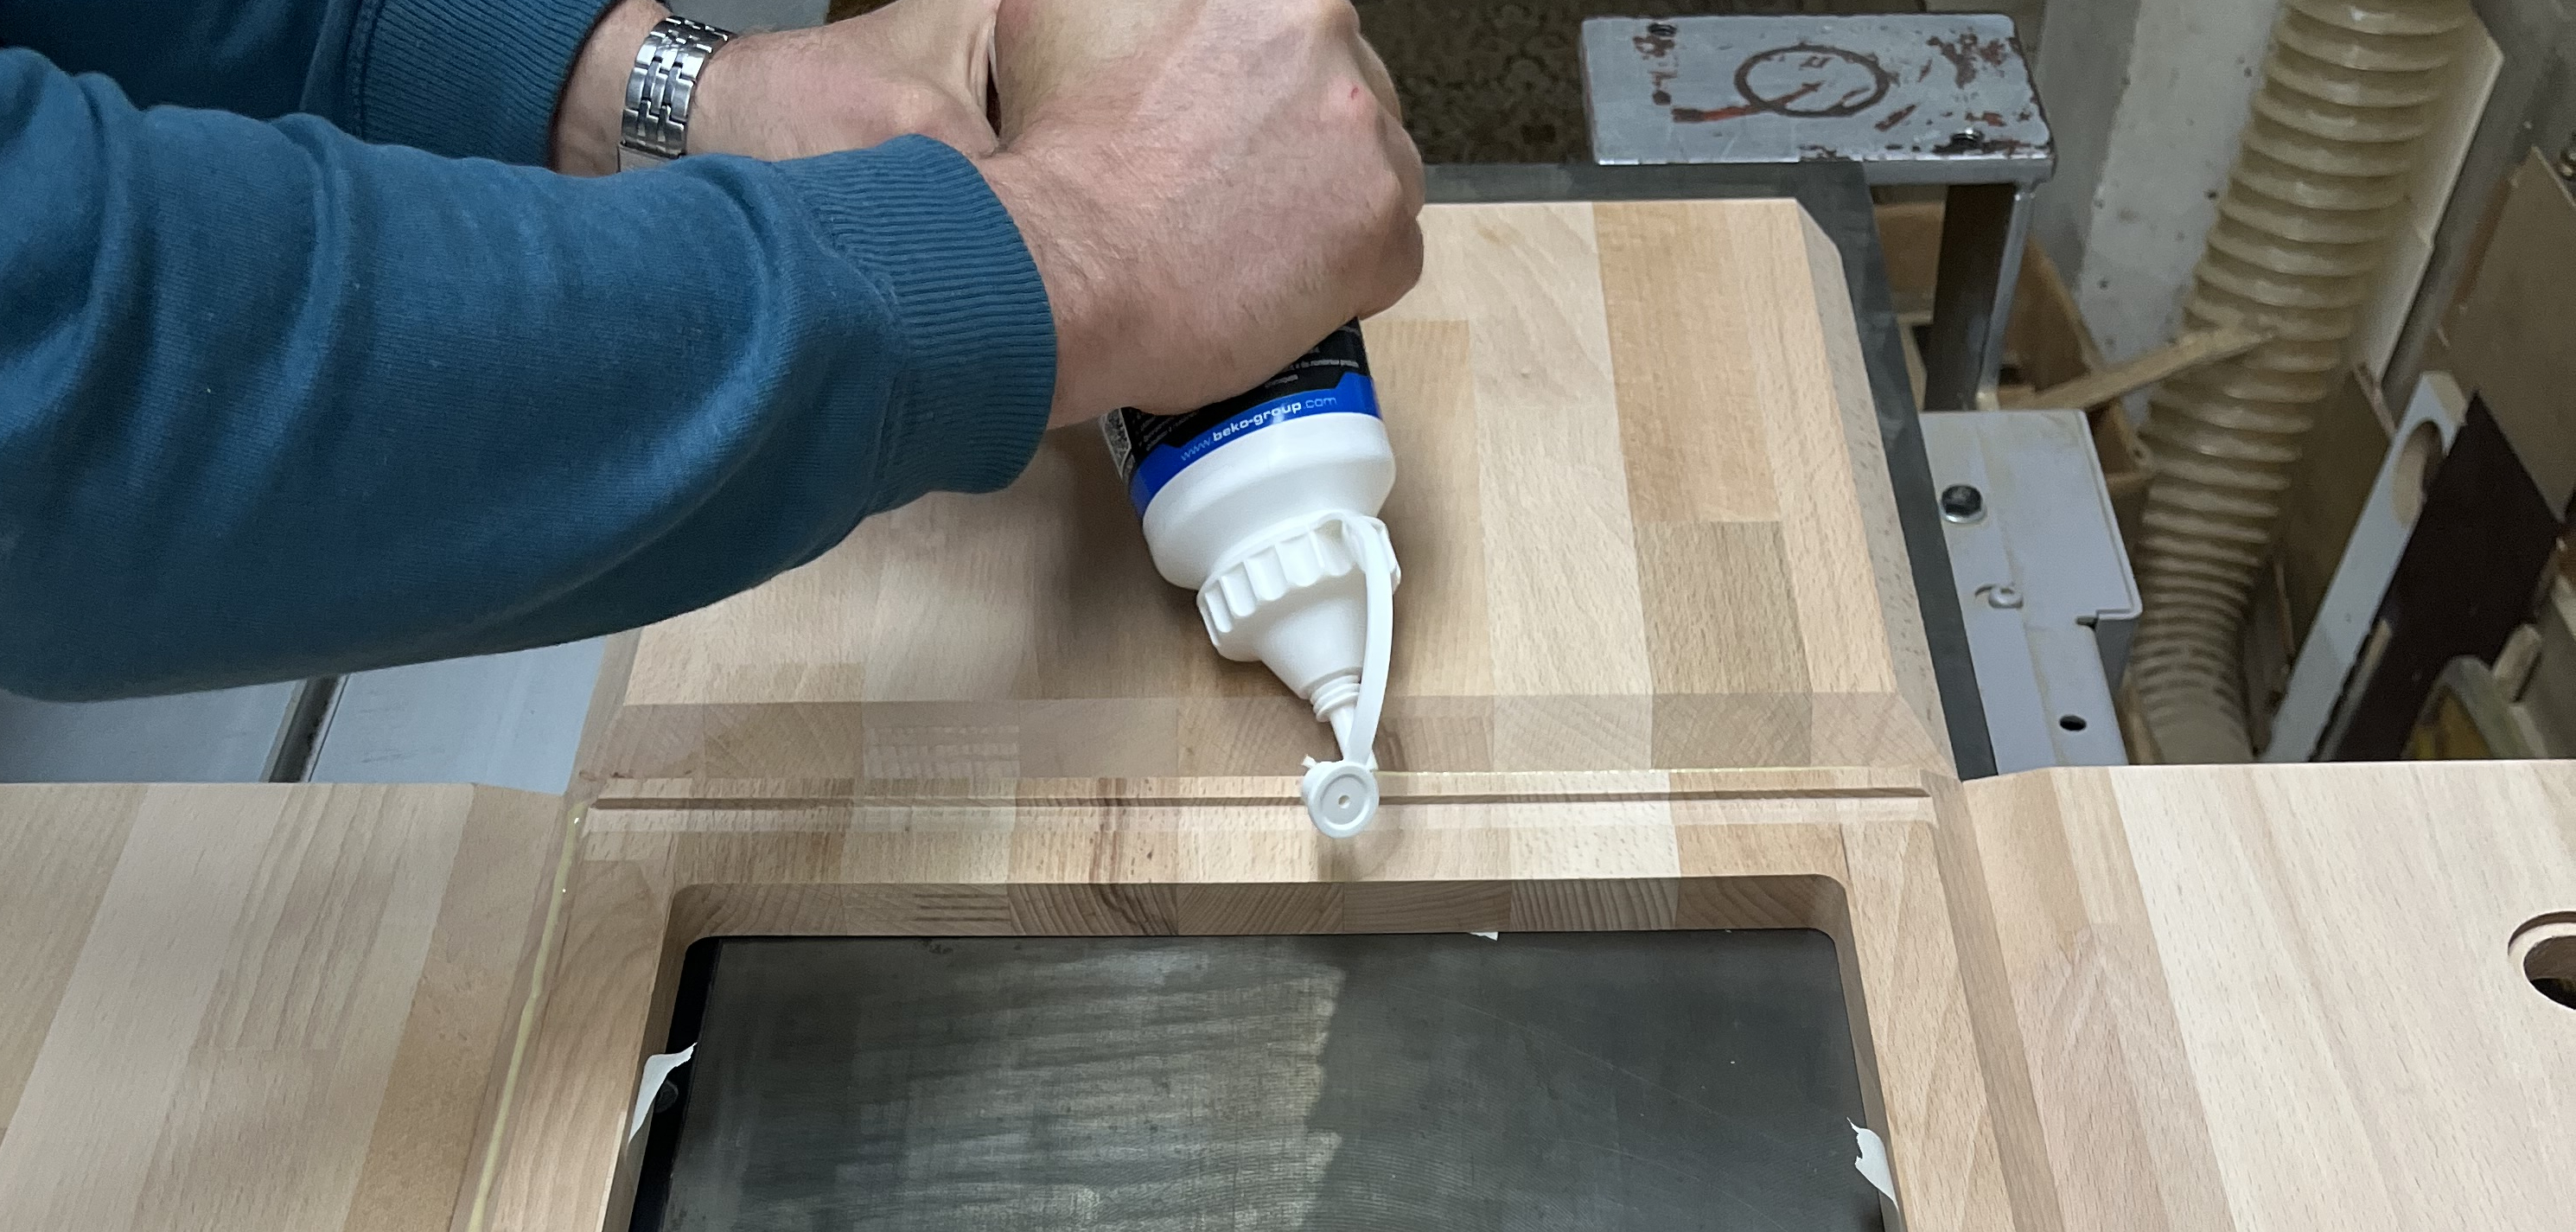
\includegraphics[width=0.75\textwidth]{fotobox_verleimen.JPG}
    \caption{Auftragen des Holzleims.}
    \label{fig:fotobox_verleimen}
\end{figure}

\newpage

Nachdem der Leim der Platten getrocknet ist, wurde das Kreppband entfernt und
alle herausquellenden Leimreste wurden entfernt. Anschließend wurden auf 
dem Frästisch alle von Vorne sichtbaren Kanten mit einem Kantenfräser mit einem
Radius von 8mm abgerundet. Dieser Arbeitsschritt ist in \autoref{fig:fotobox_fraesen}

\begin{figure}[H]
    \centering
    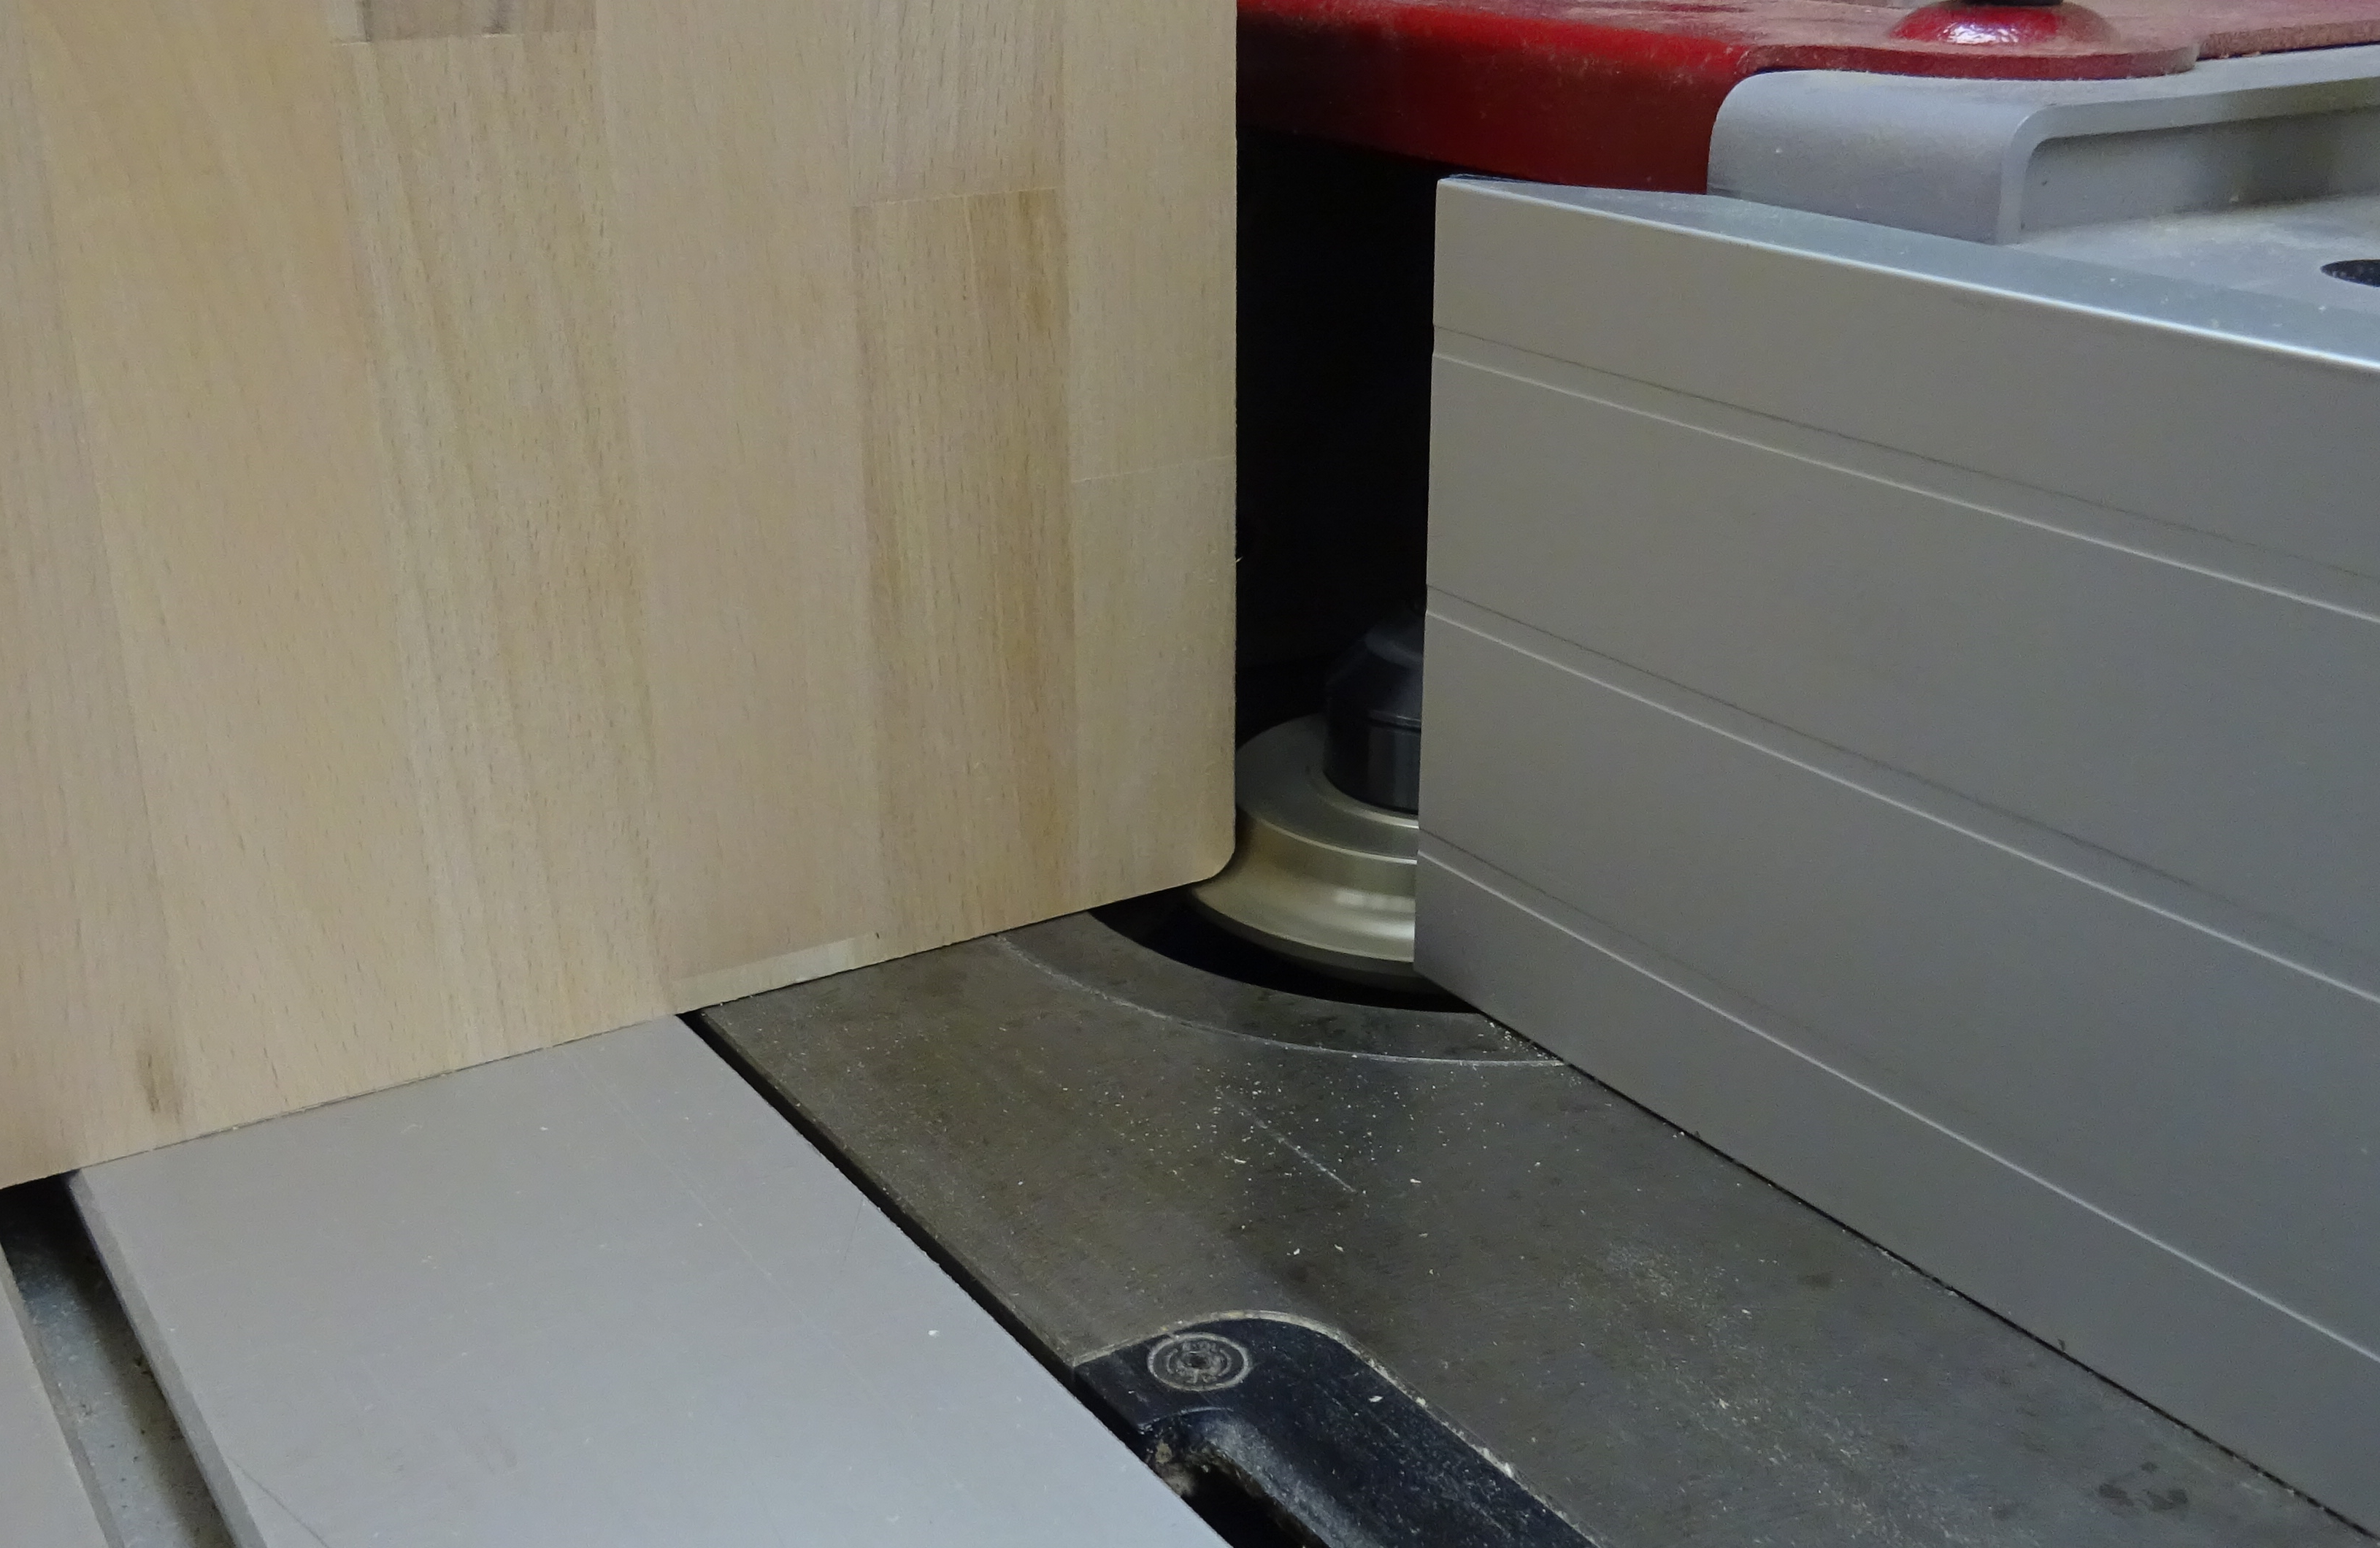
\includegraphics[width=0.75\textwidth]{kanten_fraesen.JPG}
    \caption{Fräsen der Kanten.}
    \label{fig:fotobox_fraesen}
\end{figure}

\newpage

\subsubsection{Bauen der Halterungen}

Als Nächstes wurden die Halterungen für die Kamera, den Blitz und den Laptop gebaut.


Für die Halterung des Blitzes, mussten in ein Flacheisen, zwei m6 Gewinde
eingeschnitten werden, um anschließend, dies ist in \autoref{fig:fertiges_gewinde}
zu sehen ist eine Gewindestange einzuschrauben.

\begin{figure}[H]
    \centering
    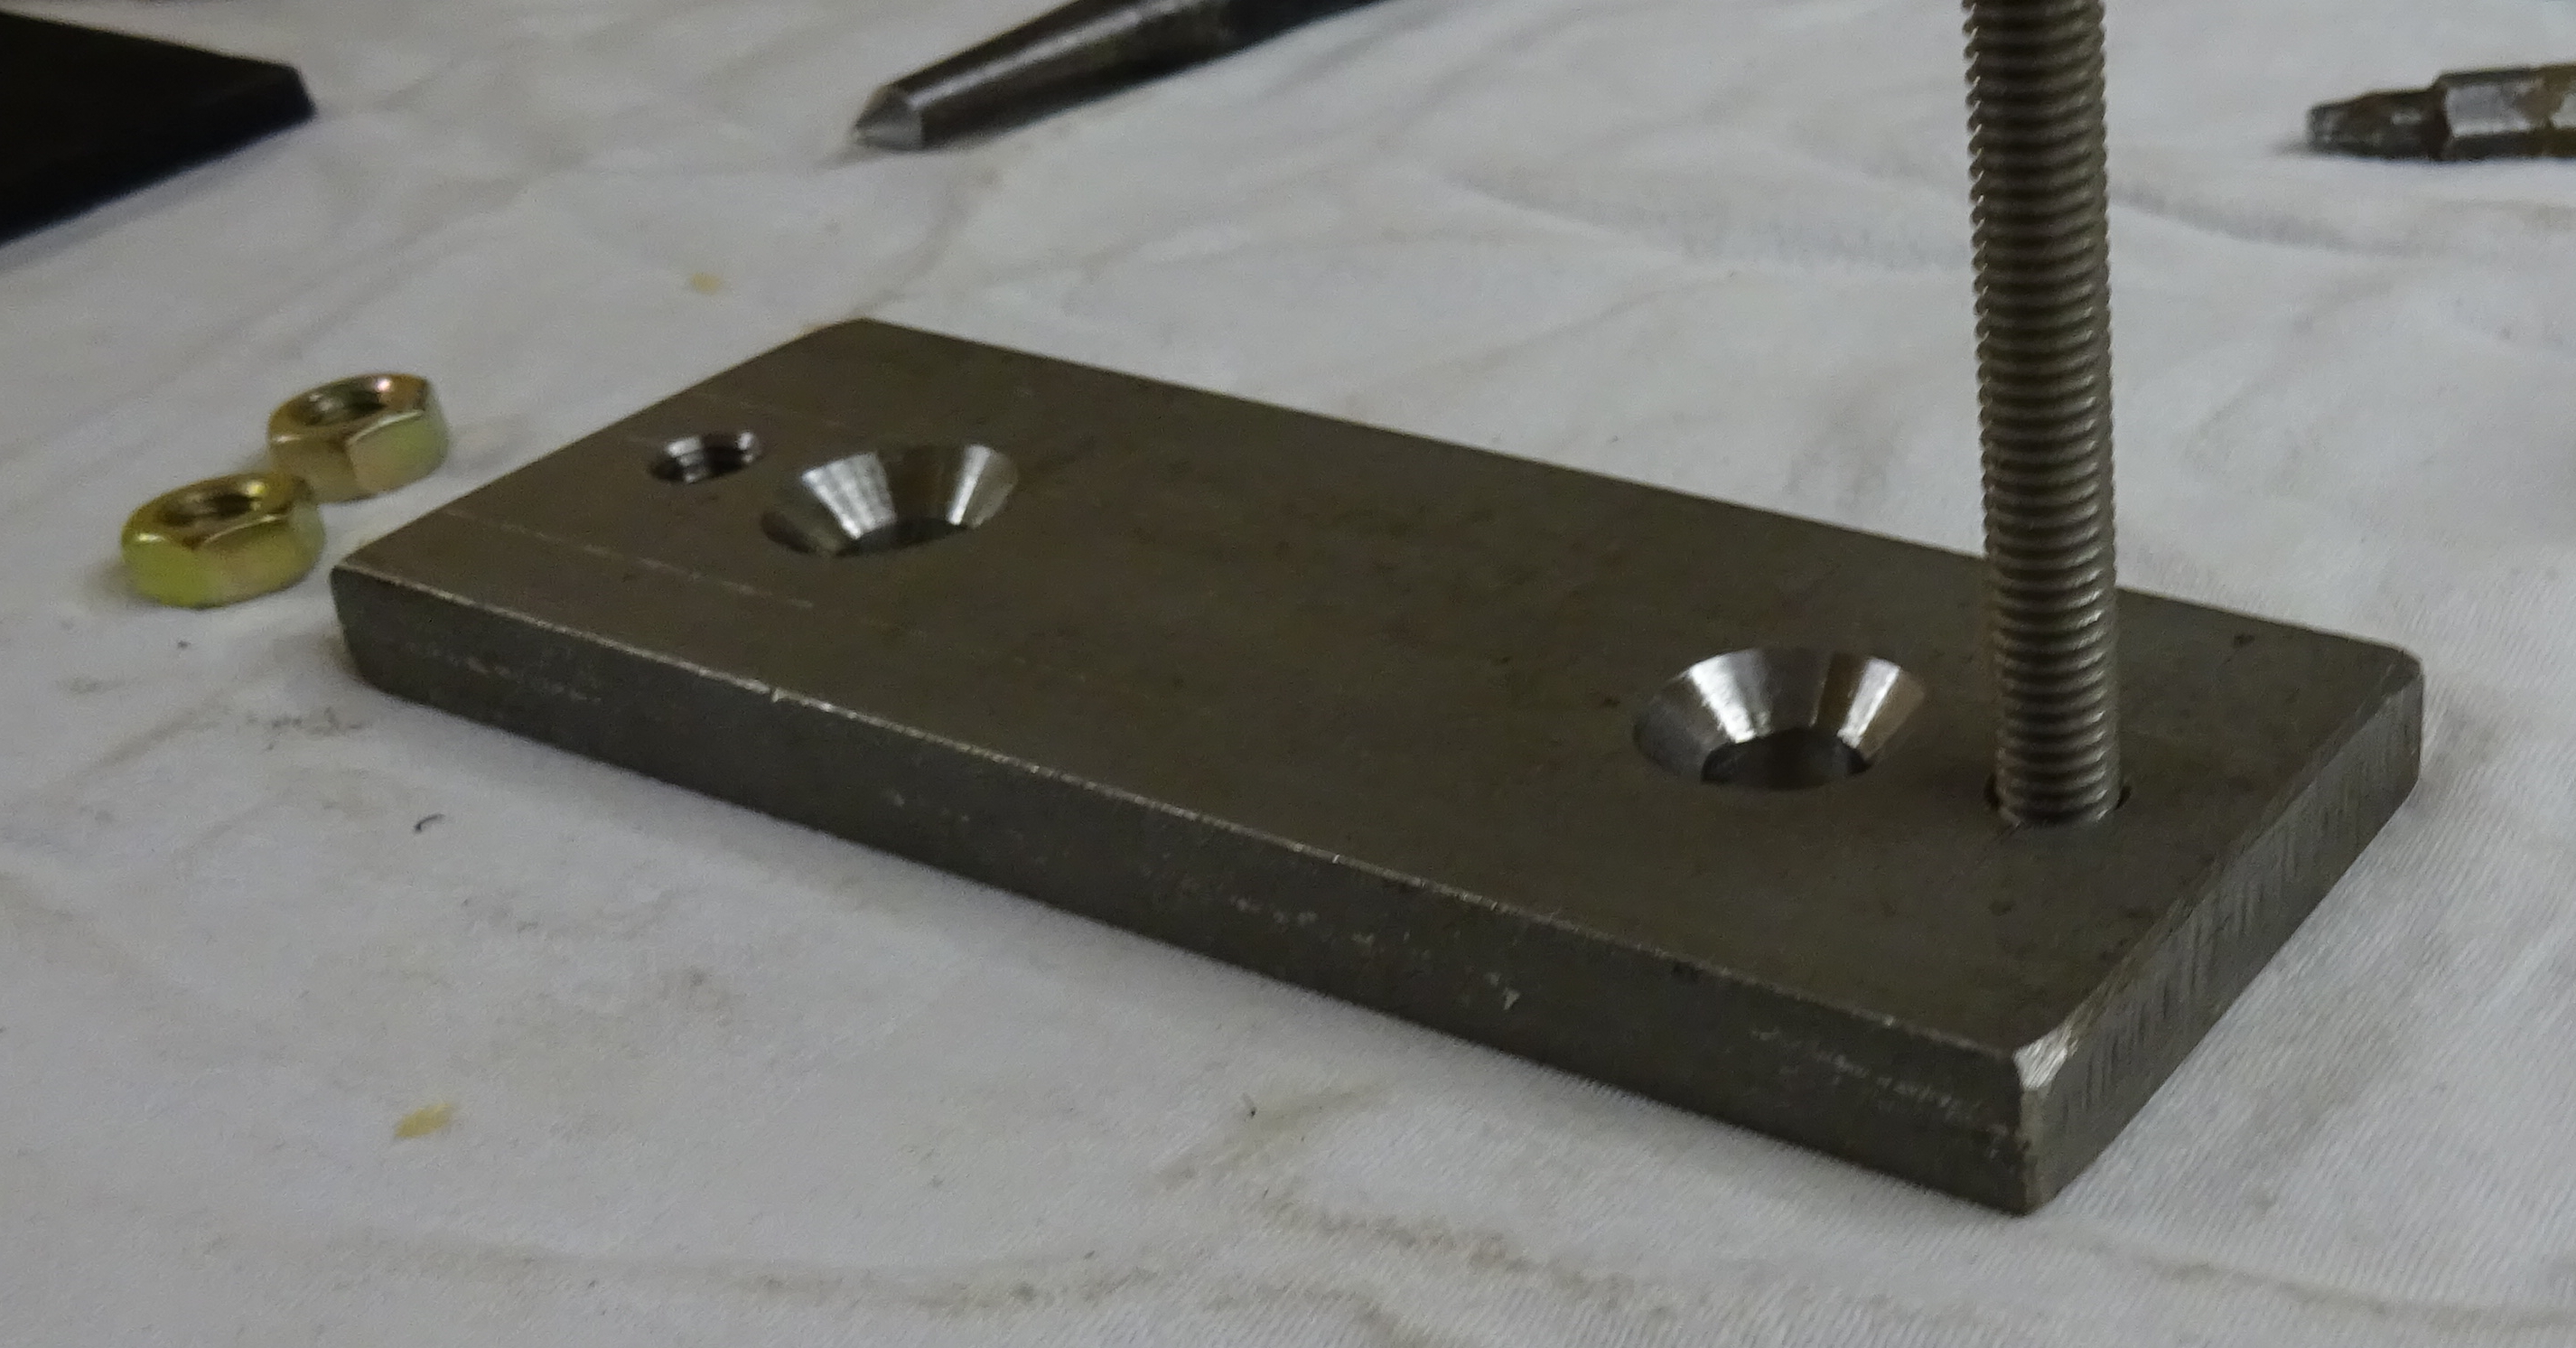
\includegraphics[width=0.75\textwidth]{fertiges_gewinde.JPG}
    \caption{Flacheisen mit Gewinde.}
    \label{fig:fertiges_gewinde}
\end{figure}

Um ein Gewinde der Größe M6 herzustellen, muss zuvor ein Kernloch mit einem
Durchmesser von 5mm gebohrt werden. Der entsprechende Arbeitsschritt wird in
\autoref{fig:loch_bohren} gezeigt.

\begin{figure}[H]
    \centering
    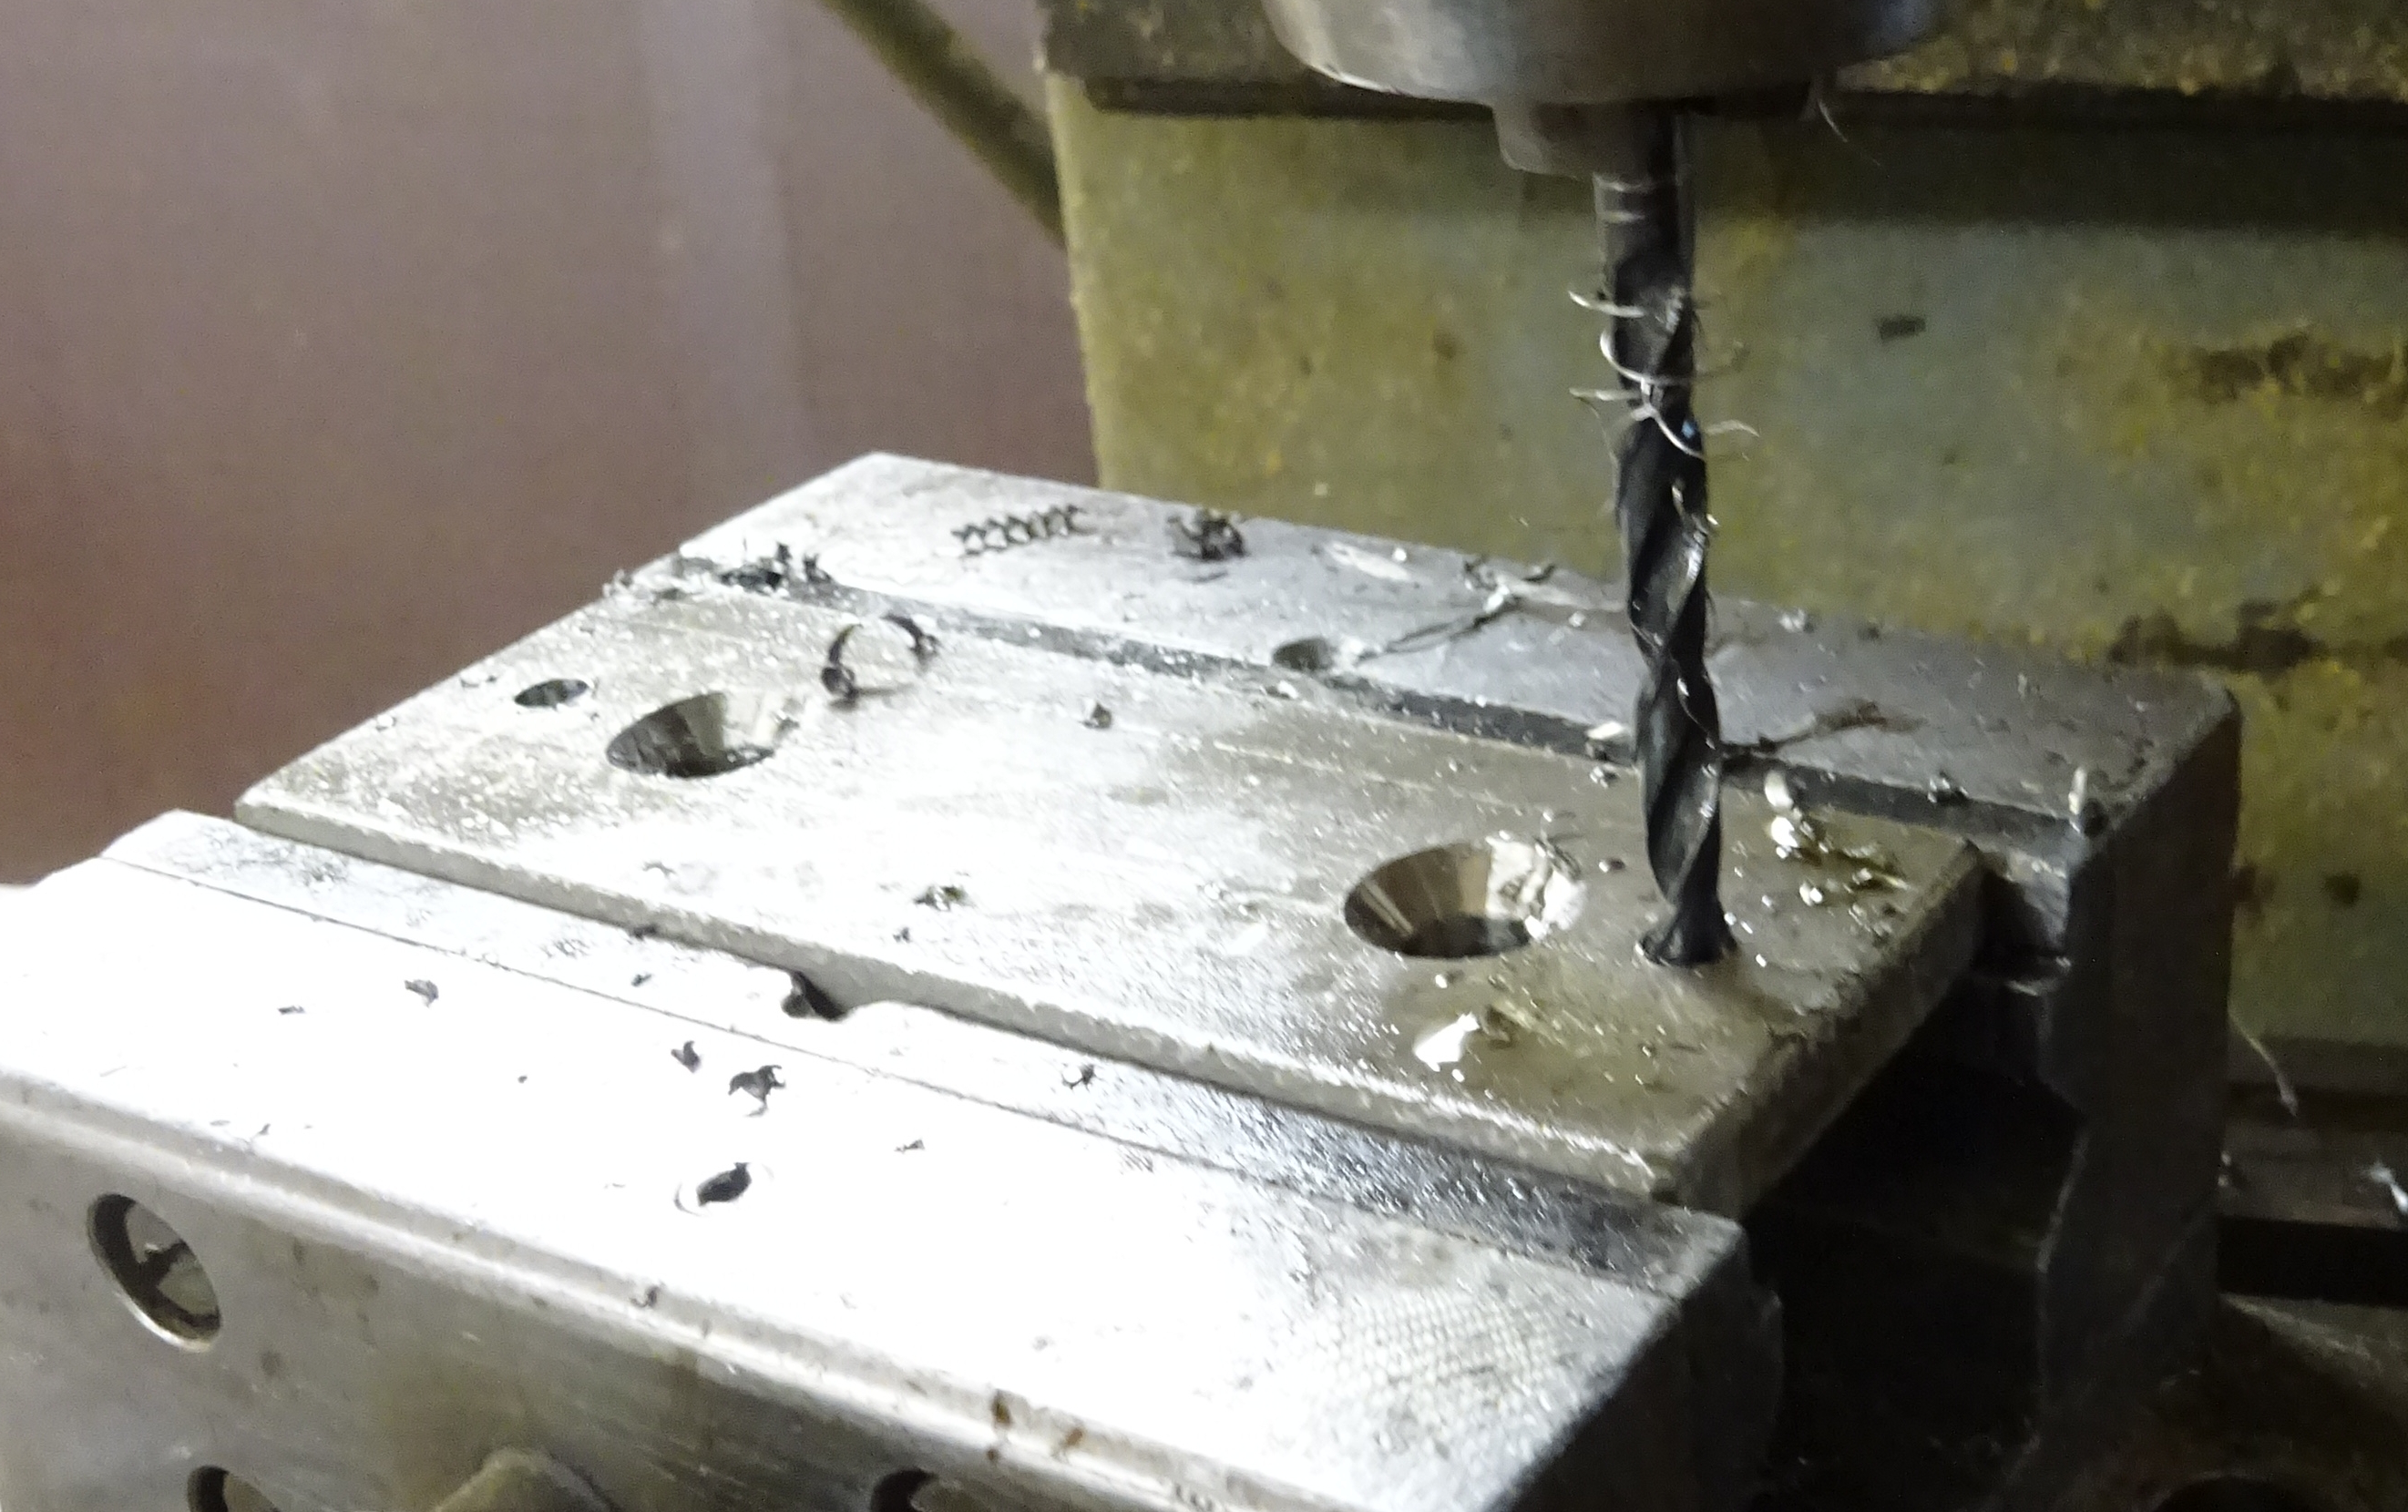
\includegraphics[width=0.75\textwidth]{loch_bohren.JPG}
    \caption{Bohren des Lockes im Flacheisen.}
    \label{fig:loch_bohren}
\end{figure}

\newpage

Anschließend wird das gebohrte Loch mit einem Kegelsenker bearbeitet, wodurch
der beim Bohren entstandene Grat entfernt wird, sichtbar in \autoref{fig:loch_senken}.

\begin{figure}[H]
    \centering
    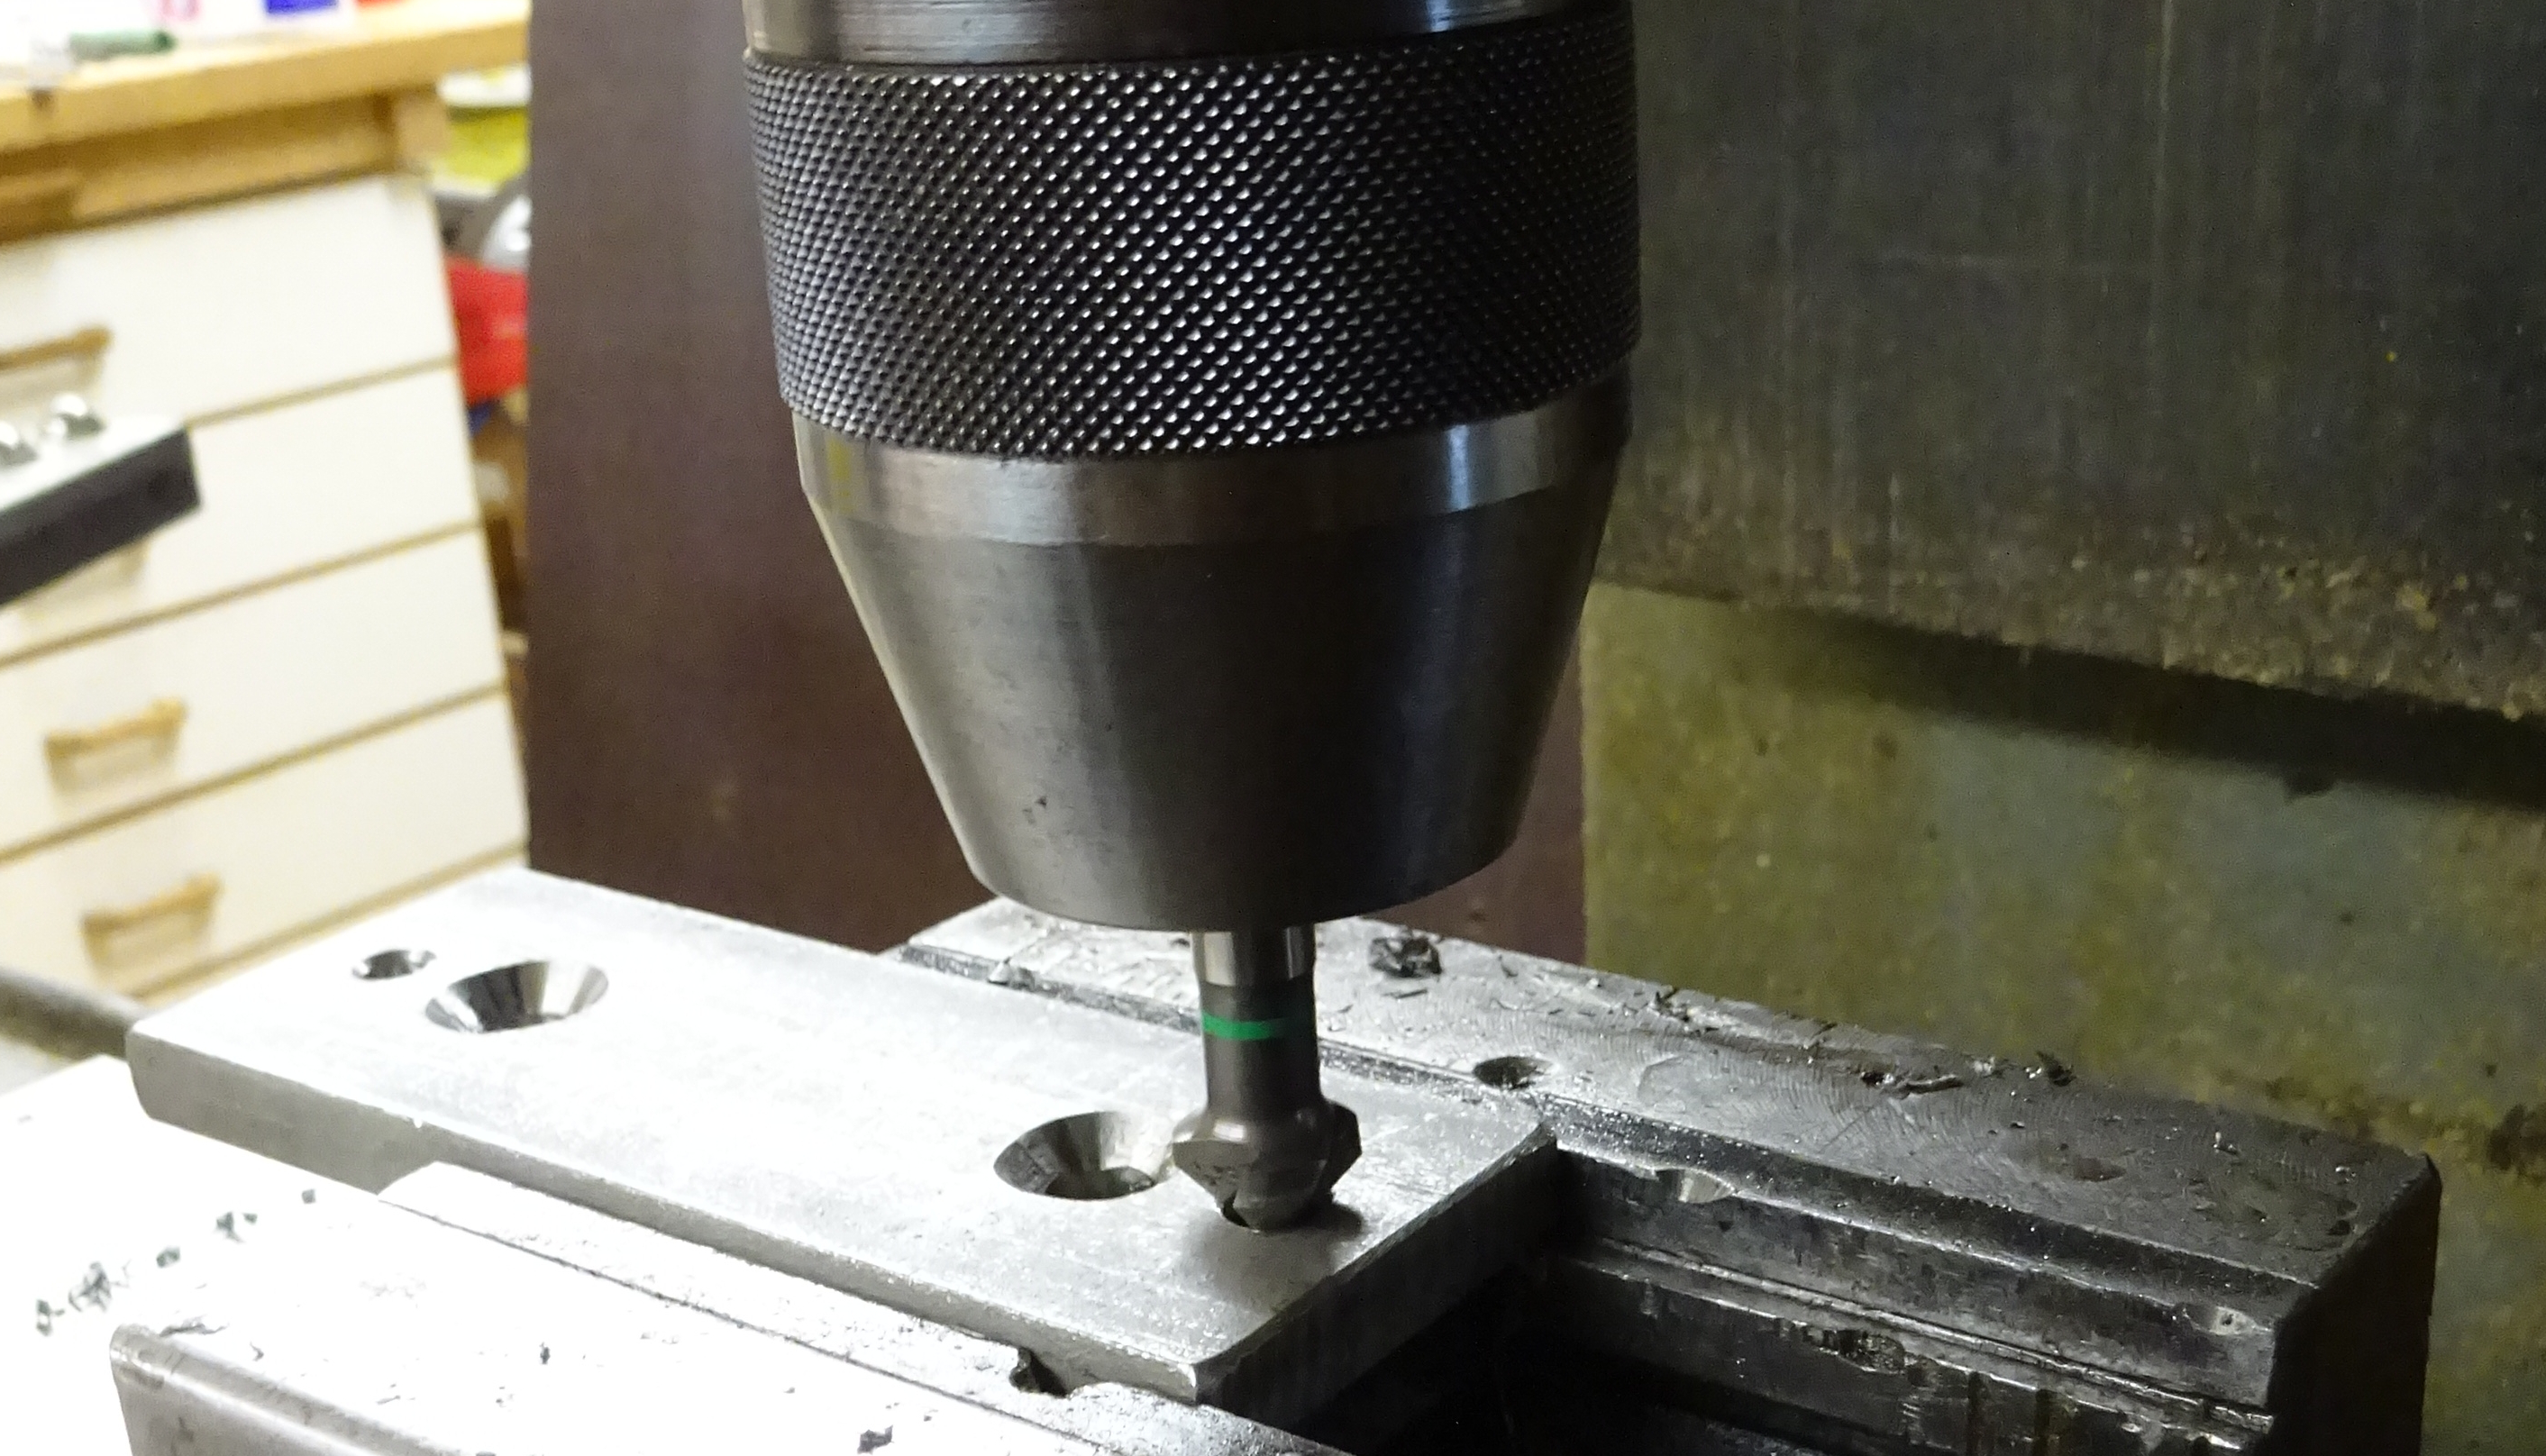
\includegraphics[width=0.75\textwidth]{loch_senken.JPG}
    \caption{Entgraten des Loches.}
    \label{fig:loch_senken}
\end{figure}

Als letzter Schritt wird nun das Gewinde mit einem Gewindeschneider geschnitten,
wie in Abbildung \autoref{fig:gewinde_schneiden} dargestellt.

\begin{figure}[H]
    \centering
    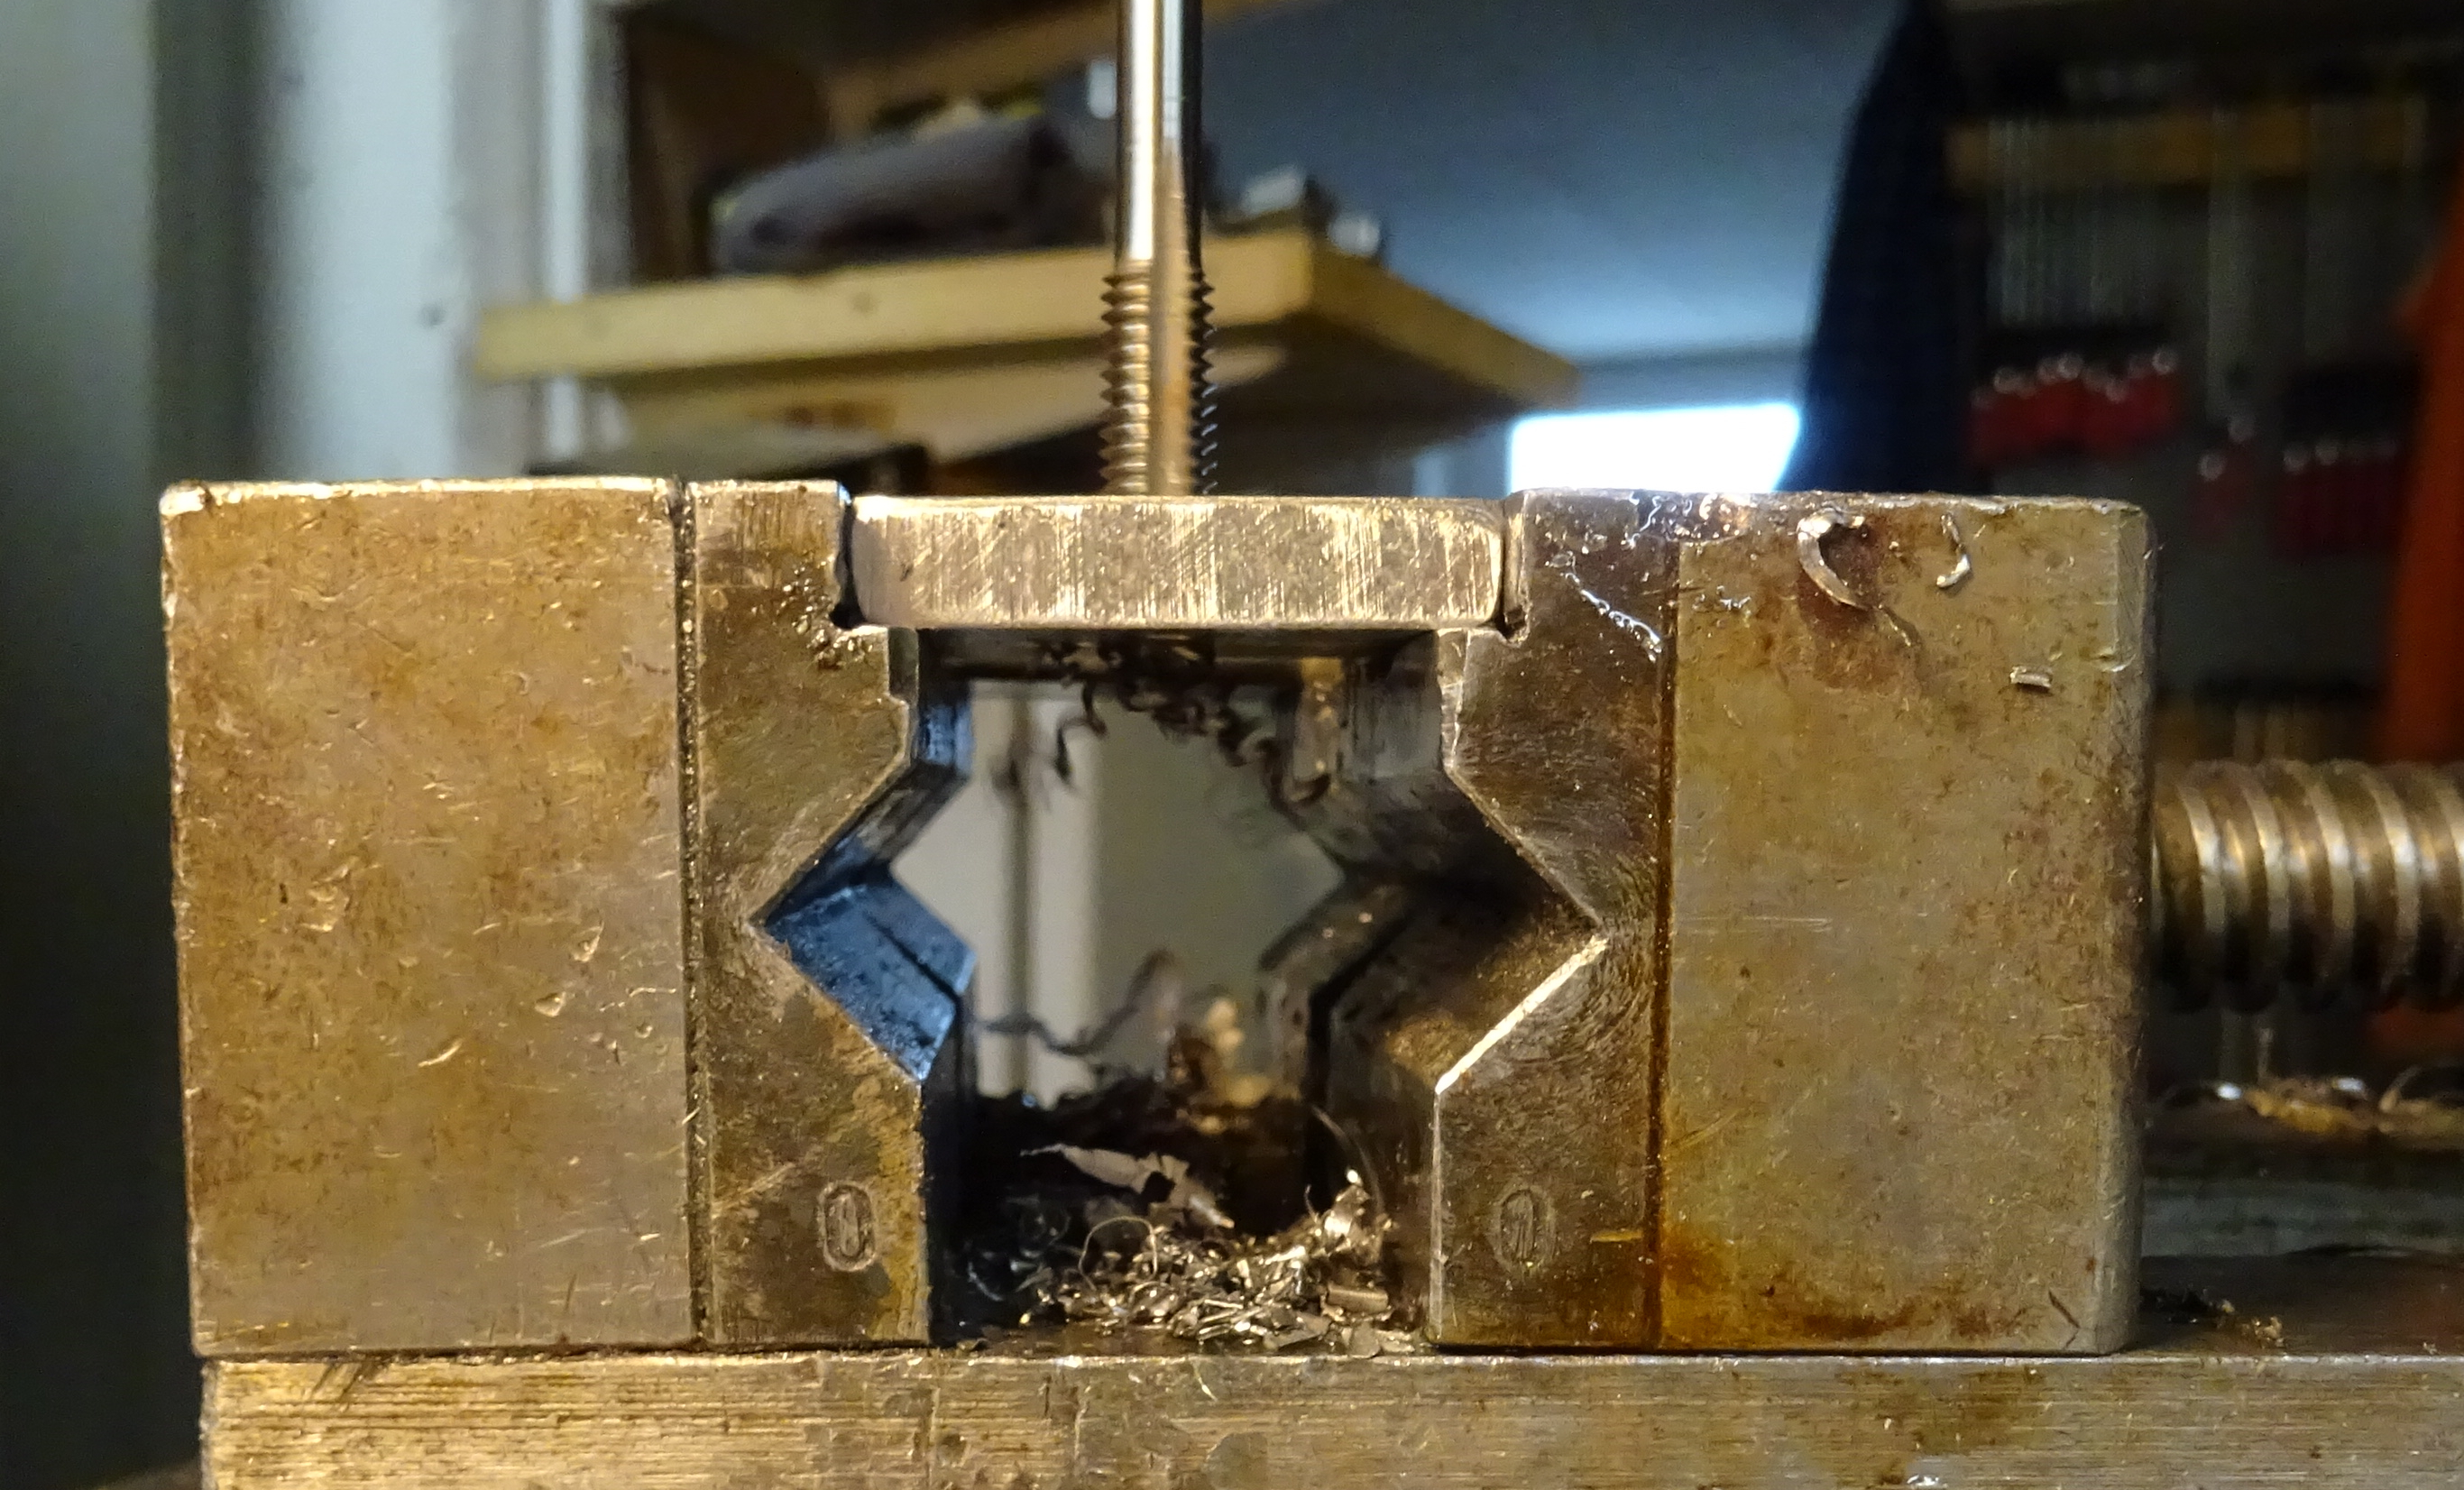
\includegraphics[width=0.75\textwidth]{gewinde_schneiden.JPG}
    \caption{Schneiden des Gewindes.}
    \label{fig:gewinde_schneiden}
\end{figure}

\newpage

Die fertige halterung 


\subsubsection{Schleifen und Ölen der Box}

Nachdem die Box zusammengeleimt, die Ecken abgerundet und die Halterungen
gebaut wurden, wurde die gesamte Oberfläche sorgfältig geschliffen.
Dabei kamen zunächst grobere Schleifpapiere zum Einsatz, um Unebenheiten zu
beseitigen und die Übergänge zwischen den verleimten Holzleisten zu glätten.
Anschließend wurde mit feineren Körnungen nachgearbeitet, um eine gleichmäßige,
glatte Oberfläche zu erzielen, die sich angenehm anfühlt und für die
anschließende Behandlung vorbereitet ist.

Nach dem Schleifen wurde die Oberfläche gründlich entstaubt,
bevor ein farbloses Holzöl aufgetragen wurde, das die natürliche Maserung
der Buche hervorhebt und gleichzeitig als Schutzschicht gegen Feuchtigkeit
und Schmutz dient. Dieser Vorgang wurde in mehreren Schichten durchgeführt,
wobei zwischen den einzelnen Aufträgen jeweils eine Trocknungszeit eingehalten wurde.


\begin{figure}[H]
    \centering
    \includegraphics[width=0.75\textwidth]{images/mechanics/fotobox_fertig.JPG}
    \caption{Die fertige Box.}
    \label{fig:gewinde_schneiden}
\end{figure}

\end{document}
